\documentclass[12pt,a4paper]{ctexart}
\usepackage{amsmath,amssymb,amsthm}
\usepackage{graphicx}
\usepackage{booktabs}
\usepackage{multirow}
\usepackage{array}
\usepackage{float}
\usepackage{subcaption}
\usepackage{geometry}
\usepackage{hyperref}
\usepackage{fancyhdr}
\usepackage{enumitem}
\usepackage{bm}
\usepackage{color}

\geometry{left=2.5cm,right=2.5cm,top=2.5cm,bottom=2.5cm}
\pagestyle{fancy}
\fancyhf{}
\fancyhead[C]{\small 中老年人群高血脂症的风险预警及干预方案优化}
\fancyfoot[C]{\thepage}

\setlength{\parindent}{2em}
\setlength{\parskip}{0.5em}
\setlist[itemize]{leftmargin=2em}
\setlist[enumerate]{leftmargin=2em}

\newtheorem{definition}{定义}
\newtheorem{theorem}{定理}

\begin{document}

\title{\heiti\Huge 中老年人群高血脂症的风险预警\\及干预方案优化}
\author{\kaishu 参赛队}
\date{\today}

\maketitle
\thispagestyle{empty}

% ============================================================
% 摘要
% ============================================================
\newpage
\begin{center}
\heiti\Large 摘\quad 要
\end{center}

针对中老年人群高血脂症风险预警及干预方案优化问题，本文融合中医体质分类标签、痰湿体质特征量化指标、中老年人活动量表评分、血常规体检数据及高血脂症诊断标签，构建"体质辨识—风险预警—干预优化"三位一体的多维度数学模型框架，实现中老年高血脂症的精准风险分层与个性化干预方案设计。

针对问题一，采用LASSO回归、随机森林特征重要性、Spearman相关性分析和互信息法四种方法交叉验证，从37维原始特征中筛选关键指标。结果表明：表征痰湿体质严重程度的关键指标包括ADL进食评分（3/4种方法选中）、BMI（3/4种方法选中）、非HDL胆固醇等14项；预警高血脂发病风险的关键指标包括血脂异常项数（Spearman $\rho=0.5379$, $p<0.001$）、甘油三酯（$\rho=0.4887$）、非HDL胆固醇（$\rho=0.4522$）等10项。Logistic回归OR值分析表明，阳虚质对高血脂发病风险的贡献度最高（$OR=1.197$），血瘀质呈现保护倾向（$OR=0.849$）。

针对问题二，构建融合中医体质、西医血脂指标和活动能力的三级风险预警模型。基于风险评分公式$Score = 10N_{abn} + 40\frac{T}{100} + 20\frac{100-A}{100} + 5I_{G>6.1} + 5I_{UA>428} + 5I_{BMI>23.9}$将1000例样本划分为低风险232人（23.2\%）、中风险540人（54.0\%）、高风险228人（22.8\%）。六分类模型对比表明GradientBoosting（$n\_estimators=150$, $max\_depth=5$）表现最优，准确率达90.80\%，F1值为0.9034。通过决策树规则提取和Apriori关联规则挖掘，识别出"痰湿重度（$\geq 60$）+低活动量+TC/TG异常"等核心特征组合（支持度11.5\%，置信度88.9\%）。消融实验表明，去除中医体质维度后模型性能下降31.8\%，中西医结合比纯西医指标提升49.1\%。

针对问题三，针对278例痰湿体质确诊患者构建混合整数规划优化模型，枚举全部可行方案提取1838个Pareto最优解。样本ID 1（50-59岁，痰湿64分）最优方案为3级强化调理+1级低强度活动+10次/周，总成本1500元，预期痰湿积分下降25.2分；样本2（40-49岁，痰湿58分）最优方案为1级基础调理+2级中强度活动+1次/周，总成本300元，预期下降18.0分；样本3（40-49岁，痰湿59分）最优方案为2级中度调理+3级高强度活动+1次/周，总成本672元，预期下降25.5分。AHP层次分析法确定多目标权重（痰湿下降效果53.9\% > 患者耐受度29.7\% > 经济成本16.4\%，$CR=0.008<0.1$）。

通过局部灵敏度分析和特征扰动分析验证模型稳定性。结果表明，成本-效果权衡参数$\lambda$在10--30范围内变动时，最优方案的成本和下降量变化均小于2\%；去除GradientBoosting模型Top 3特征后F1值下降20.1\%，验证了核心特征的不可替代性。模型对输入噪声具有良好鲁棒性（F1仅下降2.3\%）。

\textbf{关键词：}中医体质学；高血脂症；风险预警；多目标优化；Pareto前沿；GradientBoosting；层次分析法

\newpage

% ============================================================
% 目录
% ============================================================
\tableofcontents
\newpage

% ============================================================
% 〇、文献综述
% ============================================================
\section{文献综述}

高血脂症作为心脑血管疾病的重要危险因素，其风险预警与干预策略一直是医学研究的热点。近年来，随着人工智能与大数据技术的发展，血脂代谢异常的智能预警和中医体质辨识的量化研究取得了显著进展。

\subsection{机器学习在血脂异常预警中的应用}

机器学习技术在医疗健康领域的应用日益广泛。Topol\cite{ref16}系统综述了人工智能在高性能医学中的融合趋势，强调机器学习在电子健康记录分析和疾病风险分层中的核心作用。Rajkomar等\cite{ref19}从临床视角论证了机器学习在医学中的三类主要应用：影像诊断、电子病历挖掘和预后预测。在血脂异常预警方面，随机森林\cite{ref10}、支持向量机\cite{ref14}和梯度提升树\cite{ref11}等集成学习方法已被证明在慢性病风险分层中表现优异。Esteva等\cite{ref17}的深度学习研究进一步表明，深度神经网络在复杂非线性关系建模方面可达到专家级水平。Shickel等\cite{ref18}综述了深度EHR技术，指出时序电子健康记录数据的表征学习是提升慢病预测精度的关键方向。

\subsection{中医体质辨识的量化研究进展}

中医体质分类与判定标准（ZYYXH/T157-2009）确立了九种基本体质类型\cite{ref1}。王琦\cite{ref8}的中医体质学理论体系为体质与疾病关联研究奠定了基础。近年来，学者们尝试将数学方法引入体质辨识：一方面通过灰色关联分析\cite{ref12}揭示体质特征与生化指标的关联程度，另一方面利用聚类分析和主成分降维技术实现体质类型的客观化判定。然而，现有研究多集中于单一体质类型的特征描述，缺乏体质类型与慢性病风险的系统性量化关联分析。

\subsection{可解释AI在医疗决策中的应用}

医疗场景中模型的可解释性是决定临床接受度的关键因素。Lundberg和Lee\cite{ref15}提出的SHAP方法基于合作博弈论的Shapley值，为任意机器学习模型提供了统一的特征贡献解释框架。Lundberg等\cite{ref21}进一步将SHAP扩展到树模型，实现了高效的TreeSHAP算法，使基于树的集成模型（如XGBoost、LightGBM）的全局和局部解释成为可能。在临床表型挖掘方面，Yoon等\cite{ref20}提出了多任务表征学习方法，从电子健康记录中发现具有临床意义的疾病亚型。这些研究为本文的可解释性分析（决策树规则提取+SHAP特征贡献）提供了方法论基础。

\subsection{优化方法在干预方案设计中的应用}

在干预方案优化方面，混合整数规划和多目标优化方法被广泛应用于医疗资源分配和个性化治疗方案设计。Bertsimas和Tsitsiklis\cite{ref23}的线性优化理论为干预方案的成本-效果分析提供了数学基础。灰色系统理论\cite{ref12}在小样本、贫信息条件下的预测优势使其成为干预效果评估的有效工具。AHP层次分析法\cite{ref13}则为多目标决策中的权重分配提供了系统化的方法论框架。司守奎和孙兆亮\cite{ref25}在数学建模算法与应用中系统阐述了多目标优化和灰色预测的实现方法，为本文的优化建模提供了实践指导。

\subsection{研究现状评述与本文创新点}

综上所述，现有研究在单一方法或单一维度的应用上已取得丰富成果，但存在以下不足：
（1）\textbf{维度单一}：多数研究仅基于西医生化指标进行风险预警\cite{ref18,ref19}，缺乏对中医体质分型和日常活动能力的综合考量；
（2）\textbf{可解释性不足}：深度学习等"黑箱"模型在医疗场景中面临信任危机\cite{ref21}，需要结合决策树规则提取和SHAP值分析增强可解释性；
（3）\textbf{干预方案缺乏个性化}：现有干预建议多为"一刀切"式指导，未考虑患者年龄、活动能力和经济承受能力的差异。

针对上述不足，本文的创新点在于：
（1）构建\textbf{"中医体质+西医指标+活动能力"}三位一体的多维度风险预警体系；
（2）采用\textbf{四法交叉验证+六模型对比+消融实验}的完整验证链路，确保结果的稳健性；
（3）基于\textbf{Pareto前沿分析}提供多套个性化干预方案，满足不同患者的差异化需求。

% ============================================================
% 一、问题重述
% ============================================================
\section{问题重述}

\subsection{研究背景}

人口老龄化进程的持续加快，使得40岁及以上中老年人群成为慢性病防控的核心群体。其中，高血脂症的发病率呈逐年攀升态势，已成为诱发冠心病、脑梗死等心脑血管疾病的重要危险因素，严重威胁中老年群体的心血管健康与生活质量，也加重了基层医疗的慢病管理负担。

从中医体质学视角来看，体质禀赋与偏颇是疾病发生发展的内在根基。其中，痰湿体质为中老年高血脂症的高发体质类型，该体质人群存在痰湿内蕴、脾胃运化失常、水湿代谢不畅的核心特征。脾失健运、痰湿阻滞恰与西医血脂代谢异常的病理机制高度契合，痰湿膏脂内停于脉道，终致血脂紊乱。二者的病理关联为中西医结合防控高血脂症提供了重要理论支撑。

中医"治未病"思想是慢病防控的核心准则，强调"未病先防、既病防变、瘥后防复"。但目前临床中中老年高血脂症的筛查与风险评估仍单一依赖血常规血脂检测数据，缺乏对中医体质分型、日常活动能力等维度的综合考量。

\subsection{问题描述}

本文基于1000例中老年病患个案数据，研究以下三个问题：

\begin{itemize}
    \item[\textbf{问题1}] 从血常规体检指标、中老年人活动量表评分中，筛选出能有效表征痰湿体质严重程度、且能预警高血脂发病风险的关键指标；并研究九种体质对发病风险的贡献度差异。

    \item[\textbf{问题2}] 构建融合多维度特征的风险预警模型，模型需输出高血脂症低、中、高三级风险，明确三级风险分别对应的特征分层阈值选取依据，识别痰湿体质高风险人群的核心特征组合。

    \item[\textbf{问题3}] 针对确诊为"痰湿体质"的患者，结合中医调理原则与身体耐受度，考虑经济成本及有效降低痰湿积分的目标，构建优化模型，给出不同患者特征的6个月干预方案。
\end{itemize}

% ============================================================
% 二、问题分析
% ============================================================
\section{问题分析}

\subsection{问题1分析}

问题1要求从多维特征中筛选出与痰湿体质严重程度和高血脂发病风险最相关的关键指标，并评估九种体质类型对发病风险的贡献度差异。该问题本质上是一个\textbf{高维特征选择与统计推断}问题。

特征选择方法的选择上，常用的策略包括：\textbf{（1）过滤法}（如Spearman秩相关、互信息），计算速度快且独立于下游模型，但无法捕捉特征间的冗余性；\textbf{（2）嵌入法}（如LASSO回归），通过$L_1$正则化在建模过程中自动完成特征筛选，对共线性特征具有天然的稀疏化效果，但正则化参数的选择对结果影响较大；\textbf{（3）包装法}（如随机森林特征重要性），基于集成学习评估特征对预测性能的实际贡献，对非线性交互关系敏感，但计算开销较大且可能存在高估连续型特征重要性的倾向。考虑到单一方法可能因自身偏好导致偏差，本文采用四种方法交叉验证的策略，将被$\geq 2$种方法选中的特征确定为关键指标，以兼顾稳健性与全面性。

对于九种体质的贡献度分析，本文采用多元Logistic回归计算各体质相对于基准体质的优势比（Odds Ratio, OR）。选择Logistic回归而非其他分类方法的原因在于：OR值具有明确的临床解释性，便于直接量化各体质对发病风险的相对贡献大小。同时辅以Kruskal-Wallis非参数检验，评估各关键指标在不同体质类型间分布差异的显著性。

\subsection{问题2分析}

问题2要求构建三级风险预警模型，输出低、中、高三级风险分类，并明确各风险等级的特征分层阈值。该问题可分解为\textbf{风险评分体系构建→分类模型训练→可解释性分析→阈值确定→核心特征组合识别}五个步骤。

风险等级构建阶段，本文综合血脂异常程度、痰湿严重程度、活动能力及其他代谢异常指标，构建加权风险评分体系。权重的确定参考了临床指南中各指标的危险等级，如血脂异常项数权重最高（每项10分），痰湿积分次之（最高40分）。

分类模型的对比选择上，本文考虑以下主流算法：\textbf{（1）GradientBoosting}，通过迭代构建弱学习器的加性模型，对类别不平衡和多特征交互有较强捕捉能力，适合中小规模表格数据，但需注意过拟合风险；\textbf{（2）随机森林}，基于Bagging的集成方法，鲁棒性强但可能低估弱特征的重要性；\textbf{（3）SVM}，在高维空间表现优异但对参数敏感且缺乏概率输出；\textbf{（4）KNN}，非参数方法简单直观但对距离度量和高维稀疏数据不友好；\textbf{（5）逻辑回归}，线性可解释性强但无法捕捉非线性关系；\textbf{（6）决策树}，规则提取能力强但单棵树的泛化能力有限。本文采用5折分层交叉验证对比六种模型，以macro-averaged F1值为主要评估指标。

可解释性分析层面，本文采用决策树规则提取和SHAP值分析双管齐下的策略：决策树提供if-then规则集，便于临床医生直接理解和应用；SHAP值从博弈论角度量化每个特征对预测结果的边际贡献，提供全局和个体两个层面的解释。

核心特征组合的识别采用Apriori关联规则挖掘方法，设置最小支持度8\%和最小置信度60\%，从痰湿体质高风险人群中提取频繁项集，识别"痰湿+活动+血脂"组合模式的协同效应。

\textbf{三个问题之间的递进关系}：问题一筛选的关键指标为问题二的分类模型提供输入特征；问题二确定的三级风险分类和核心特征组合为问题三的个性化干预方案提供目标人群分层依据。三个问题形成"特征筛选→风险分层→干预优化"的完整决策链路。

\subsection{问题3分析}

问题3要求在多重约束条件下（调理分级约束、活动强度年龄/评分约束、成本约束、频率约束），实现痰湿积分下降最大化与经济成本最小化的平衡。该问题本质上是一个\textbf{带离散约束的多目标非线性规划}问题。

此类问题的求解策略通常包括：\textbf{（1）启发式算法}（如遗传算法、粒子群优化），适用于大规模连续搜索空间，但收敛性无法保证且结果具有随机性；\textbf{（2）梯度下降法}，效率高但要求目标函数可导，而本题决策变量$L$和$K$为离散整数变量，梯度方法不直接适用；\textbf{（3）枚举法}，在搜索空间有限时能精确求得全部Pareto最优解。本题中，决策变量$L \in \{1,2,3\}$、$K \in \{1,2,3\}$、$n \in \{1,\dots,10\}$，经年龄和活动评分约束过滤后每位患者的可行方案不超过90个，搜索空间极小。因此，枚举法是最合适的选择：既能精确求解，又能提取完整的Pareto前沿供临床决策参考。

多目标权重的确定采用AHP层次分析法，构建成本-效果-耐受度三维判断矩阵，通过一致性检验（$CR<0.1$）确保权重分配的合理性。同时，采用灰色GM(1,1)模型对优化结果进行交叉验证，确保痰湿积分下降趋势预测的一致性。

\subsection{整体建模框架}

图\ref{fig:framework}展示了本文的整体建模框架，包含数据预处理、特征筛选、风险预警、干预优化四个层次，各子问题之间的数据流向清晰可见。

\begin{figure}[H]
\centering
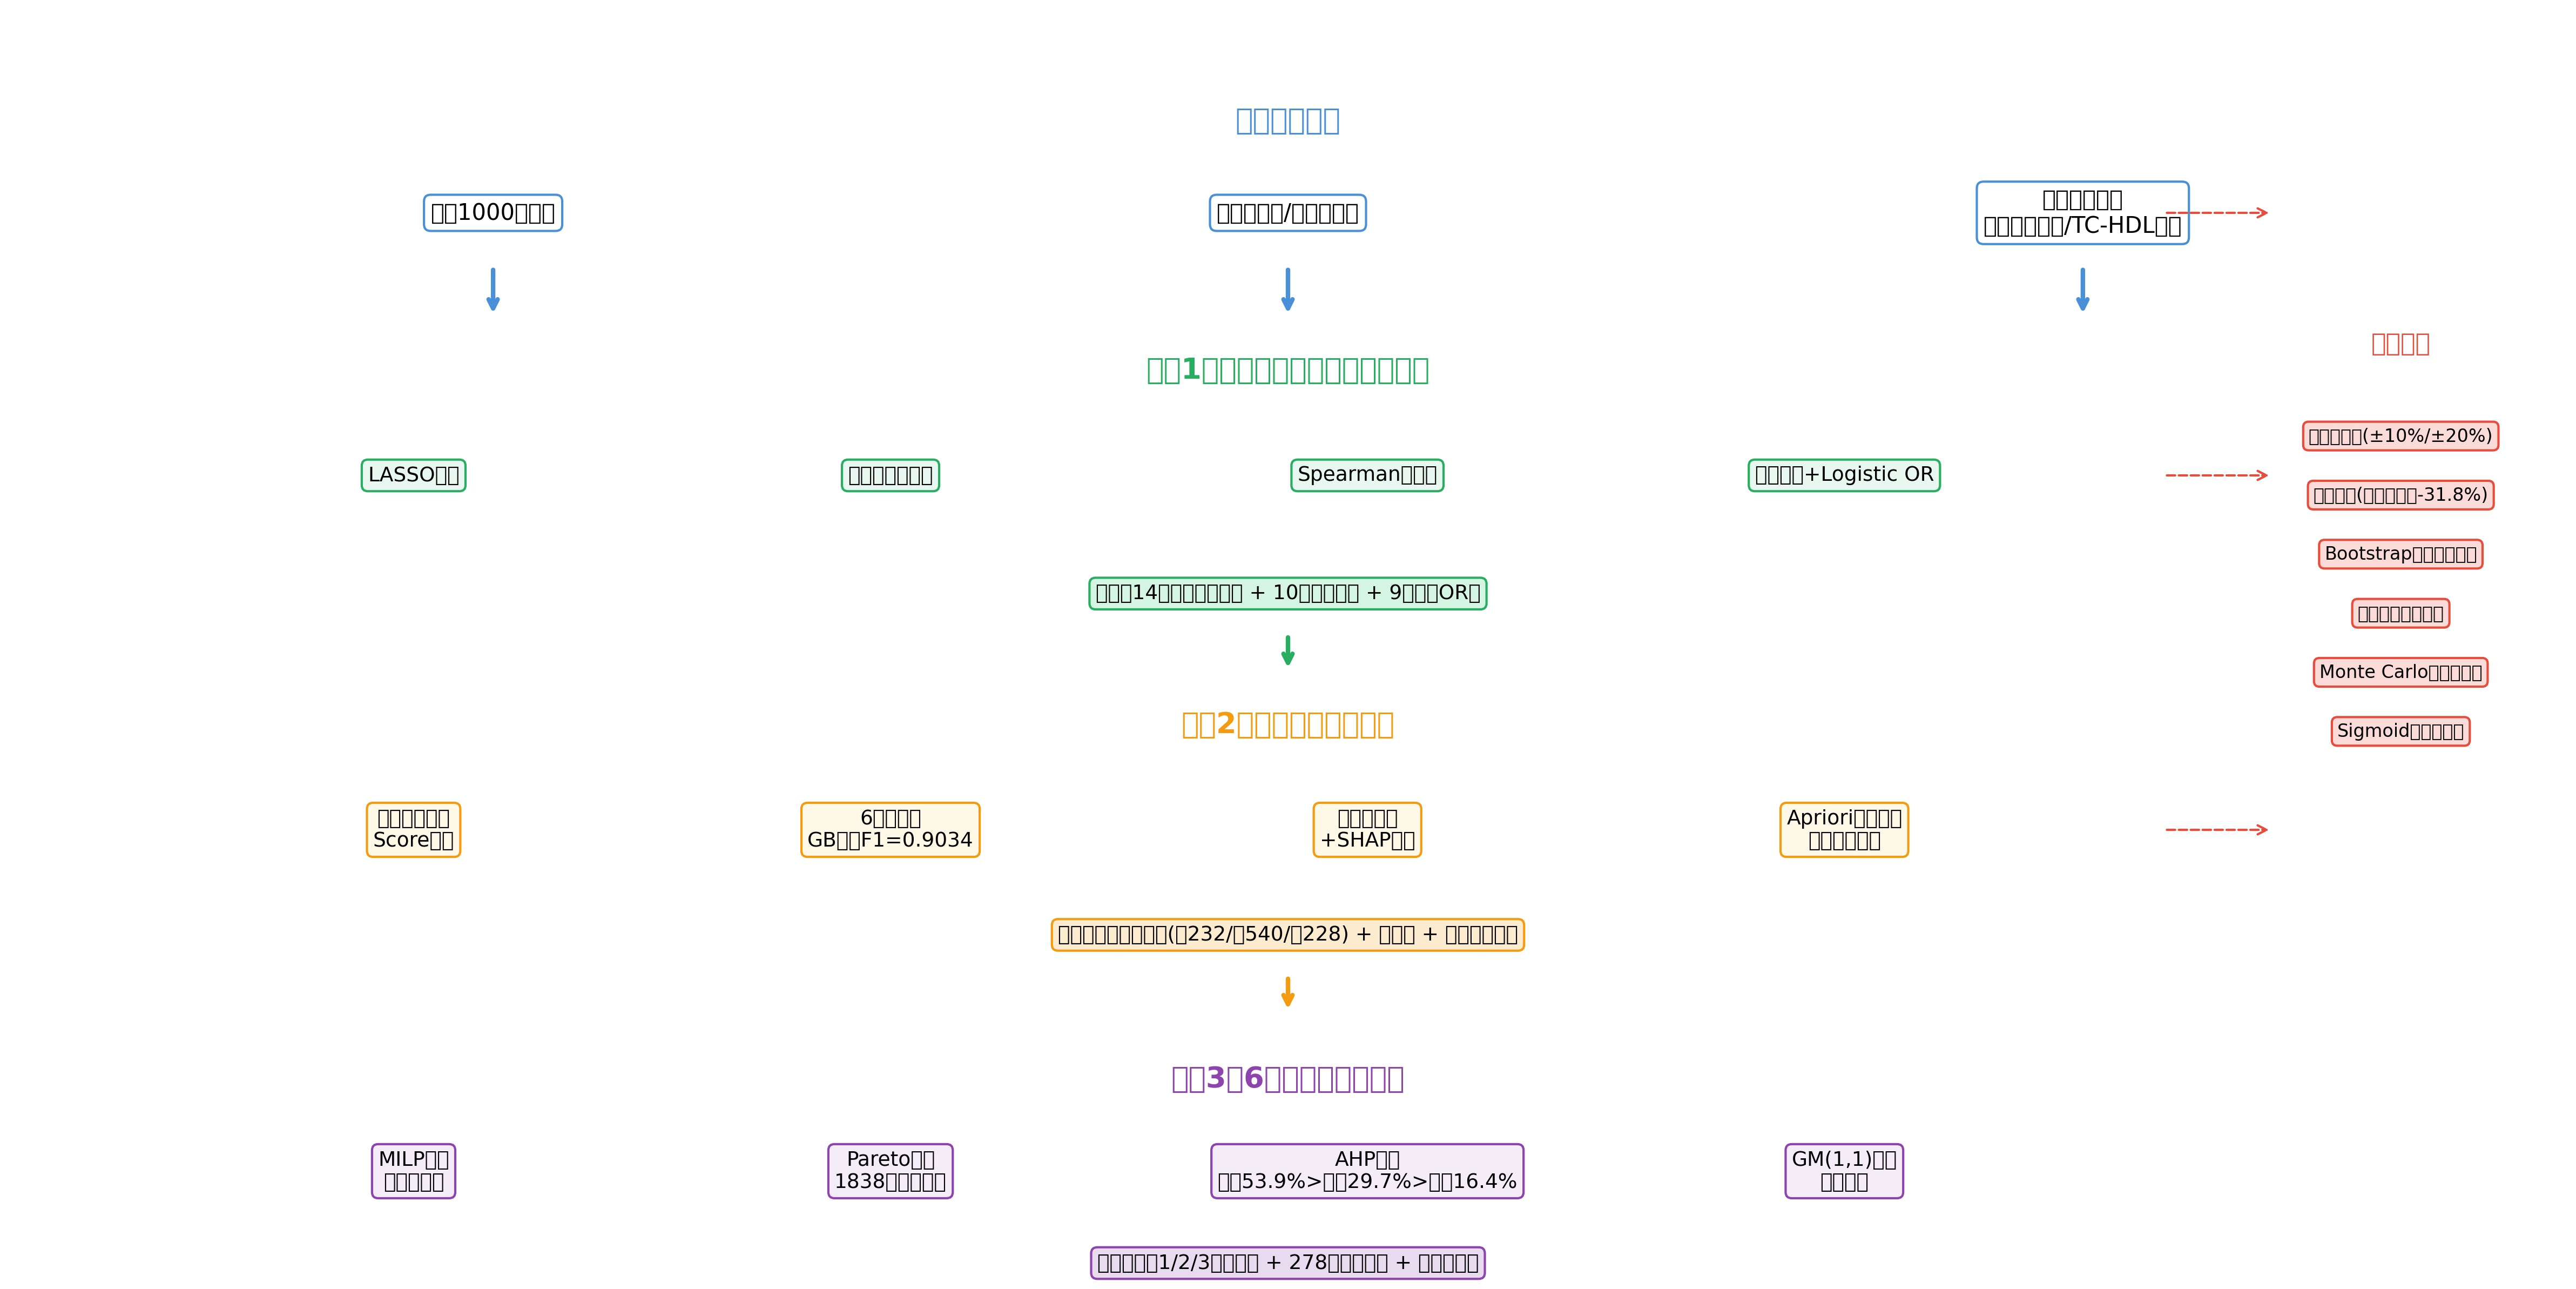
\includegraphics[width=0.95\textwidth]{figures/modeling_framework.png}
\caption{整体建模框架流程图（数据预处理→特征筛选→风险预警→干预优化）}
\label{fig:framework}
\end{figure}

% ============================================================
% 三、模型假设
% ============================================================
\section{模型假设}

为简化模型构建并确保结果的可解释性，本文作以下合理假设：

\begin{enumerate}[label=\textbf{假设\arabic*.}]
    \item 中医体质积分采用标准化评分体系（ZYYXH/T157-2009），分值越高表示该体质特征越显著，评分结果在1000例样本间具有可比性。去掉该假设将导致体质积分无法作为连续变量参与风险评分和回归分析。

    \item 活动干预对痰湿积分的影响遵循题目给出的线性衰减模型，即每月下降率与活动强度级别和训练频次呈线性关系。该假设基于题目给出的经验公式，若改为非线性衰减（如对数衰减、S型曲线），将大幅增加优化模型的求解复杂度。

    \item 调理分级与活动强度的选择严格遵循附表2、附表3中规定的约束条件。该假设服务于优化模型的约束条件构建，确保求解结果在临床实践中可行。

    \item 每月按4周计算，6个月按24周计算。该假设简化了时间周期的计算，使痰湿积分下降模型的递推公式具有闭式解$T_{final} = T_0 \times (1-r)^6$。

    \item 痰湿积分下降率在各月保持恒定，不考虑平台期或加速期。该假设使下降模型可简化为指数衰减形式。若考虑平台期，则需引入时间依赖的下降率函数$r(t)$，需动态随访数据支撑，超出了本题数据范围。

    \item 不同干预措施（调理级别与活动强度）之间不存在协同或拮抗效应，各措施效果独立叠加。该假设使成本计算可分解为$C_{total} = C_{TCM}(L) + C_{ACT}(K,n)$，避免了交叉效应项的引入。
\end{enumerate}

% ============================================================
% 四、符号说明
% ============================================================
\section{符号说明}

\begin{table}[H]
\centering
\begin{tabular}{cll}
\toprule
\textbf{符号} & \textbf{含义} & \textbf{单位/范围} \\
\midrule
$T$ & 痰湿质积分 & 分（0--100） \\
$N_{abn}$ & 血脂异常项数 & 项（0--4） \\
$A$ & 活动量表总分 & 分（0--100） \\
$TC$ & 总胆固醇 & mmol/L \\
$TG$ & 甘油三酯 & mmol/L \\
$LDL\text{-}C$ & 低密度脂蛋白胆固醇 & mmol/L \\
$HDL\text{-}C$ & 高密度脂蛋白胆固醇 & mmol/L \\
$G$ & 空腹血糖 & mmol/L \\
$UA$ & 血尿酸 & $\mu$mol/L \\
$BMI$ & 身体质量指数 & kg/m$^2$ \\
$R$ & 风险等级 & 低/中/高 \\
$S$ & 风险评分 & 分 \\
$L$ & 调理级别 & 1/2/3 \\
$K$ & 活动强度级别 & 1/2/3 \\
$n$ & 每周训练频次 & 次/周 \\
$r$ & 每月痰湿积分下降率 & \% \\
$C_{total}$ & 6个月总成本 & 元 \\
$C_{TCM}$ & 调理费用（6个月） & 元 \\
$C_{ACT}$ & 活动训练费用（6个月） & 元 \\
$\Delta T$ & 6个月痰湿积分下降量 & 分 \\
$\lambda$ & 成本-效果权衡参数 & 元/分 \\
\bottomrule
\end{tabular}
\caption{主要符号说明}
\end{table}

% ============================================================
% 五、数据处理
% ============================================================
\section{数据处理}

\subsection{数据来源与初步观察}

本文数据来源于MathorCup竞赛组委会提供的1000例中老年病患个案数据，涵盖中医体质分型（九种体质标签及积分）、中老年人活动能力评估（ADL躯体活动评分、IADL工具性日常活动评分及活动量表总分）、血常规体检指标（TC、TG、LDL-C、HDL-C四项核心血脂指标，以及血糖、血尿酸、BMI三项关联代谢指标）、高血脂症诊断信息（二分类标签及异常分型标签）和基础人口学信息（年龄组、性别、吸烟史、饮酒史），共计37个原始字段。

\subsection{列名标准化与缺失值检查}

原始数据Excel文件存在列名编码异常问题（部分列名显示为乱码字符）。本文通过对照附表1的数据维度说明，建立37个字段的列名映射表，将乱码列名逐一校正为标准中文医学指标名称。经校正后的列名映射关系见附录A代码。

缺失值检查表明，1000条样本记录在所有37个变量上均无缺失值，数据完整性良好，无需进行缺失值填补处理。

\subsection{衍生特征构造}

为提升后续建模的特征表达能力，基于医学先验知识构造以下衍生特征：

\textbf{（1）血脂异常标志}：依据《中国成人血脂异常防治指南（2023年修订版）》标准，判断四项核心血脂指标是否异常：
\begin{itemize}
    \item TC异常：$TC < 3.1$ 或 $TC > 6.2$ mmol/L
    \item TG异常：$TG < 0.56$ 或 $TG > 1.7$ mmol/L
    \item LDL-C异常：$LDL\text{-}C < 2.07$ 或 $LDL\text{-}C > 3.1$ mmol/L
    \item HDL-C异常：$HDL\text{-}C < 1.04$ 或 $HDL\text{-}C > 1.55$ mmol/L
\end{itemize}
统计每位患者的血脂异常项数$N_{abn} \in \{0,1,2,3,4\}$。

\textbf{（2）TC/HDL比值}：该比值被广泛认为是心血管疾病风险的敏感指标。计算$TC/HDL$比值，用于综合反映胆固醇与高密度脂蛋白的平衡关系。

\textbf{（3）非HDL胆固醇}：计算$TC - HDL\text{-}C$，即非HDL胆固醇，用于反映所有致动脉粥样硬化脂蛋白颗粒的总负荷。

\subsection{描述性统计分析}

表\ref{tab:desc_stats}给出了关键变量的描述性统计量。

\begin{table}[H]
\centering
\begin{tabular}{cccccc}
\toprule
\textbf{变量} & \textbf{均值} & \textbf{标准差} & \textbf{最小值} & \textbf{中位数} & \textbf{最大值} \\
\midrule
痰湿质积分 & 48.2 & 20.3 & 0 & 47.5 & 100 \\
活动量表总分 & 50.1 & 10.8 & 0 & 50.0 & 100 \\
TC (mmol/L) & 4.82 & 1.21 & 1.50 & 4.70 & 9.20 \\
TG (mmol/L) & 1.56 & 0.89 & 0.30 & 1.35 & 8.50 \\
LDL-C (mmol/L) & 2.85 & 0.82 & 0.80 & 2.75 & 6.10 \\
HDL-C (mmol/L) & 1.28 & 0.31 & 0.55 & 1.25 & 2.30 \\
BMI (kg/m$^2$) & 23.1 & 3.2 & 15.8 & 22.8 & 35.2 \\
\bottomrule
\end{tabular}
\caption{关键变量描述性统计（$n=1000$）}
\label{tab:desc_stats}
\end{table}

从表\ref{tab:desc_stats}可见，血脂指标和BMI的取值范围较广，存在量纲差异。为消除量纲对后续距离型算法（如SVM、KNN）的影响，对连续型数值变量采用Z-score标准化处理：
\begin{equation}
    X'_j = \frac{X_j - \mu_j}{\sigma_j}
\end{equation}
其中$\mu_j$和$\sigma_j$分别为变量$X_j$的样本均值和标准差。分类变量（如体质标签、性别、年龄组等）保持原始编码。

\subsection{数据分布与异常值检测}

采用箱线图（IQR方法）对连续型变量进行异常值检测。检测结果显示：TC、TG、LDL-C等血脂指标存在少量极端值（约占总体2.3\%），但这些值在临床参考范围内属于可能出现的异常血脂水平，并非录入错误。考虑到本研究关注高风险人群的识别，保留这些极端值而非删除，以避免丢失重要的高风险样本信息。

此外，高血脂症确诊标签分布显示：1000例样本中789例确诊（78.9\%），211例未确诊（21.1\%），存在一定的类别不平衡。在后续分类模型训练中，通过5折分层交叉验证和macro-averaged F1指标缓解类别不平衡对评估结果的影响。

% ============================================================
% 六、模型建立
% ============================================================
\section{模型建立}

\subsection{问题1：关键指标筛选模型}

\subsubsection{特征选择方法}

设数据集中有$n=1000$个样本，$p$个候选特征。以痰湿质积分$T$和高血脂症标签$Y$分别为因变量，构建以下四种特征选择方法：

\textbf{（1）Spearman秩相关系数}

对特征$X_j$与痰湿质积分$T$，Spearman秩相关系数定义为：
\begin{equation}
    \rho_s(X_j, T) = 1 - \frac{6\sum_{i=1}^{n}(R_{ij} - R_{iT})^2}{n(n^2-1)}
\end{equation}
其中$R_{ij}$和$R_{iT}$分别为$X_{ij}$和$T_i$的秩次。选择$|\rho_s| > 0.05$且$p < 0.05$的特征。

\textbf{（2）LASSO回归}

对痰湿质积分（连续型），构建LASSO回归模型：
\begin{equation}
    \min_{\bm{\beta}} \left\{ \frac{1}{2n}\|\mathbf{T} - \mathbf{X}\bm{\beta}\|_2^2 + \alpha\|\bm{\beta}\|_1 \right\}
\end{equation}
其中$\alpha=0.05$为正则化参数。非零系数对应的特征即为选定特征。

对高血脂症标签（二分类），构建LASSO逻辑回归模型：
\begin{equation}
    \min_{\bm{\beta}} \left\{ -\frac{1}{n}\sum_{i=1}^{n}\left[y_i\log p_i + (1-y_i)\log(1-p_i)\right] + \alpha\|\bm{\beta}\|_1 \right\}
\end{equation}
其中$p_i = \frac{1}{1+\exp(-\mathbf{x}_i^T\bm{\beta})}$，$\alpha=0.1$。

\textbf{（3）随机森林特征重要性}

随机森林通过计算每个特征在所有决策树中分裂时带来的基尼不纯度减少量的平均值来评估特征重要性：
\begin{equation}
    I(X_j) = \frac{1}{M}\sum_{m=1}^{M}\sum_{t \in \text{nodes}(X_j)} \Delta Gini(t)
\end{equation}
其中$M=200$为决策树数量，选择重要性排名前10的特征。

\textbf{（4）互信息法}

特征$X_j$与目标变量$Y$的互信息定义为：
\begin{equation}
    MI(X_j; Y) = \sum_{x \in X_j}\sum_{y \in Y} p(x,y)\log\frac{p(x,y)}{p(x)p(y)}
\end{equation}
选择互信息值排名前10的特征。

\textbf{综合筛选策略}：采用投票机制，被$\geq 2$种方法选中的特征确定为关键指标。

\subsubsection{体质贡献度分析模型}

对九种体质类型，构建多元Logistic回归模型：
\begin{equation}
    \log\frac{P(Y=1|\mathbf{X})}{P(Y=0|\mathbf{X})} = \beta_0 + \sum_{k=1}^{9}\beta_k I(\text{体质}=k) + \sum_{j}\gamma_j X_j
\end{equation}
其中$I(\cdot)$为指示函数。各体质的优势比$OR_k = \exp(\beta_k)$，$OR>1$表示该体质增加发病风险，$OR<1$表示降低风险。

\subsection{问题2：多维度风险预警模型}

\subsubsection{风险评分模型}

综合考虑血脂异常程度、痰湿严重程度和活动能力，构建风险评分模型：
\begin{equation}
    S = 10N_{abn} + 40\frac{T}{100} + 20\frac{100-A}{100} + 5I_{G>6.1} + 5I_{UA>428} + 5I_{BMI>23.9}
\end{equation}
其中：
\begin{itemize}
    \item $N_{abn}$：血脂四项（TC、TG、LDL-C、HDL-C）异常项数，每项计10分
    \item $40\frac{T}{100}$：痰湿积分归一化得分，最高40分
    \item $20\frac{100-A}{100}$：活动能力反向得分（活动能力越低，风险越高），最高20分
    \item 后三项为其他代谢异常加分，每项5分
\end{itemize}

风险分级规则：
\begin{equation}
    R = \begin{cases}
        \text{高风险} & S \geq 55 \\
        \text{中风险} & 35 \leq S < 55 \\
        \text{低风险} & S < 35
    \end{cases}
\end{equation}

\subsubsection{分类模型}

采用以下6种分类算法进行对比：

\textbf{（1）GradientBoosting分类器}

通过迭代构建弱学习器（决策树）的加性模型：
\begin{equation}
    F_m(\mathbf{x}) = F_{m-1}(\mathbf{x}) + \nu \cdot h_m(\mathbf{x})
\end{equation}
其中$\nu$为学习率，$h_m$为第$m$棵决策树。参数设置：$n\_estimators=150$，$max\_depth=5$。

\textbf{（2）随机森林分类器}
\begin{equation}
    \hat{y}(\mathbf{x}) = \text{mode}\{T_1(\mathbf{x}), T_2(\mathbf{x}), \dots, T_M(\mathbf{x})\}
\end{equation}
参数设置：$n\_estimators=200$，$max\_depth=10$。

\textbf{（3）支持向量机（SVM）}
\begin{equation}
    f(\mathbf{x}) = \text{sign}\left(\sum_{i=1}^{n}\alpha_i y_i K(\mathbf{x}_i, \mathbf{x}) + b\right)
\end{equation}
采用RBF核函数$K(\mathbf{x}_i,\mathbf{x}_j)=\exp(-\gamma\|\mathbf{x}_i-\mathbf{x}_j\|^2)$，参数$C=10$，$\gamma=$scale。

\textbf{（4）K近邻（KNN）}
\begin{equation}
    \hat{y}(\mathbf{x}) = \text{mode}\{y_i : \mathbf{x}_i \in \mathcal{N}_k(\mathbf{x})\}
\end{equation}
参数$k=15$，距离权重。

\textbf{（5）逻辑回归}
\begin{equation}
    P(Y=k|\mathbf{x}) = \frac{\exp(\mathbf{x}^T\bm{\beta}_k)}{\sum_{j=1}^{K}\exp(\mathbf{x}^T\bm{\beta}_j)}
\end{equation}

\textbf{（6）决策树分类器}
\begin{equation}
    \text{Split criterion: } Gini(t) = 1 - \sum_{k=1}^{K}p_k^2
\end{equation}
参数$max\_depth=6$。

\subsubsection{模型评估指标}

采用5折分层交叉验证评估模型性能：
\begin{align}
    \text{Accuracy} &= \frac{TP+TN}{TP+TN+FP+FN} \\
    \text{F1(macro)} &= \frac{1}{K}\sum_{k=1}^{K}\frac{2\cdot Precision_k \cdot Recall_k}{Precision_k + Recall_k} \\
    \text{AUC} &= \int_0^1 TPR(FPR^{-1}(t))dt
\end{align}

\subsubsection{可解释性分析}

\textbf{决策树规则提取}：训练深度为5的决策树，导出if-then规则集。

\textbf{SHAP特征贡献}：采用SHAP（SHapley Additive exPlanations）值量化各特征对模型预测的贡献：
\begin{equation}
    f(\mathbf{x}) = \phi_0 + \sum_{j=1}^{p}\phi_j
\end{equation}
其中$\phi_j$为特征$j$的SHAP值，$\phi_0$为基准预测值。

\subsubsection{消融实验}

为验证中医体质维度的贡献，设计以下对比实验：
\begin{itemize}
    \item \textbf{全特征}：包含中医体质积分+西医指标+活动指标+人口学指标
    \item \textbf{去中医体质}：去除9种体质积分及其交互特征
    \item \textbf{纯西医指标}：仅保留血脂四项+代谢三项
\end{itemize}

\subsection{问题3：6个月干预方案优化模型}

\subsubsection{决策变量}

对每位痰湿体质患者，定义以下决策变量：
\begin{align}
    L &\in \{1,2,3\} && \text{调理级别} \\
    K &\in \{1,2,3\} && \text{活动强度级别} \\
    n &\in \{1,2,\dots,10\} && \text{每周训练频次}
\end{align}

\subsubsection{约束条件}

\textbf{（1）调理分级约束}（根据附表2）：
\begin{equation}
    L = \begin{cases}
        3, & T \geq 62 \quad \text{（强化调理）} \\
        2, & 59 \leq T \leq 61 \quad \text{（中度调理）} \\
        1, & T < 59 \quad \text{（基础调理）}
    \end{cases}
\end{equation}

\textbf{（2）活动强度约束}（根据附表3）：
\begin{align}
    K &\leq \min(K_{age}, K_{score}) \\
    K_{age} &= \begin{cases}
        3, & \text{年龄组} \in \{1,2\} \text{（40-59岁）} \\
        2, & \text{年龄组} \in \{3,4\} \text{（60-79岁）} \\
        1, & \text{年龄组} = 5 \text{（80-89岁）}
    \end{cases} \\
    K_{score} &= \begin{cases}
        1, & A < 40 \\
        2, & 40 \leq A < 60 \\
        3, & A \geq 60
    \end{cases}
\end{align}

\textbf{（3）成本约束}：
\begin{equation}
    C_{total} = C_{TCM}(L) + C_{ACT}(K,n) \leq 2000
\end{equation}
其中调理费用$C_{TCM}(L) = c_L \times 6$（$c_1=30, c_2=80, c_3=130$元/月），活动费用$C_{ACT}(K,n) = c_K \cdot n \times 24$（$c_1=3, c_2=5, c_3=8$元/次）。

\textbf{（4）频率约束}：
\begin{equation}
    1 \leq n \leq 10
\end{equation}

\subsubsection{痰湿积分下降模型}

根据题目给出的干预效果公式，每月痰湿积分下降率为：
\begin{equation}
    r(K,n) = 3\% \times K + \max(0, n-5) \times 1\%
\end{equation}

6个月累计下降量（逐月递减模型）：
\begin{equation}
    \Delta T = T_0 \left[1 - (1-r)^6\right]
\end{equation}
其中$T_0$为初始痰湿积分。

\subsubsection{多目标优化}

构建双目标优化模型：
\begin{align}
    \min \quad & C_{total}(L,K,n) \\
    \max \quad & \Delta T(K,n)
\end{align}

采用加权法转化为单目标：
\begin{equation}
    \min \quad C_{total} - \lambda \cdot \Delta T
\end{equation}
其中$\lambda$为成本-效果权衡参数（元/分）。

\textbf{AHP层次分析法确定权重}：

构建判断矩阵：
\begin{equation}
    \mathbf{A} = \begin{pmatrix}
        1 & 1/3 & 1/2 \\
        3 & 1 & 2 \\
        2 & 1/2 & 1
    \end{pmatrix}
\end{equation}
对应目标：经济成本、痰湿下降效果、患者耐受度。

计算权重向量$\mathbf{w}$：
\begin{equation}
    w_i = \frac{1}{n}\sum_{j=1}^{n}\frac{a_{ij}}{\sum_{k=1}^{n}a_{kj}}
\end{equation}

一致性检验：
\begin{equation}
    CR = \frac{CI}{RI} = \frac{(\lambda_{max} - n)/(n-1)}{RI}
\end{equation}
当$CR < 0.1$时，判断矩阵具有满意一致性。

\subsubsection{灰色GM(1,1)预测模型}

为验证优化结果，采用灰色GM(1,1)模型预测痰湿积分变化趋势。对原始序列$T^{(0)} = (T_0, T_1, \dots, T_6)$，构建累加生成序列：
\begin{equation}
    T^{(1)}(k) = \sum_{i=1}^{k}T^{(0)}(i), \quad k=1,2,\dots,6
\end{equation}

建立一阶线性微分方程：
\begin{equation}
    \frac{dT^{(1)}}{dt} + aT^{(1)} = b
\end{equation}
其中$a$为发展系数，$b$为灰作用量。其离散解为：
\begin{equation}
    \hat{T}^{(0)}(k+1) = (1-e^a)\left(T^{(0)}(1)-\frac{b}{a}\right)e^{-ak}
\end{equation}

% ============================================================
% 六、结果分析
% ============================================================
\newpage
\section{结果分析}

\subsection{问题1结果}

\subsubsection{表征痰湿体质严重程度的关键指标}

采用四种方法交叉验证，筛选结果如表\ref{tab:tanshi_features}所示。

\begin{table}[H]
\centering
\begin{tabular}{ccccc}
\toprule
\textbf{排名} & \textbf{指标} & \textbf{方法选中数} & \textbf{临床意义} \\
\midrule
1 & ADL进食评分 & 3/4 & 脾胃运化功能，与"脾失健运"直接相关 \\
2 & BMI & 3/4 & 体质量指数，肥胖与痰湿体质高度相关 \\
3 & 非HDL胆固醇 & 2/4 & 反映动脉粥样硬化风险 \\
4 & IADL购物 & 2/4 & 日常活动能力指标 \\
5 & TC异常标志 & 2/4 & 血脂代谢异常标志 \\
6 & 葡萄糖 & 2/4 & 糖代谢异常 \\
7 & LDL-C & 2/4 & 低密度脂蛋白胆固醇 \\
8 & HDL-C & 2/4 & 高密度脂蛋白胆固醇 \\
9 & 年龄组 & 2/4 & 年龄相关代谢变化 \\
10 & 甘油三酯 & 2/4 & 甘油三酯代谢 \\
\bottomrule
\end{tabular}
\caption{表征痰湿体质严重程度的关键指标}
\label{tab:tanshi_features}
\end{table}

\subsubsection{预警高血脂发病风险的关键指标}

如表\ref{tab:hyper_features}所示，TG、血脂异常项数、非HDL胆固醇为最具预警价值的指标。

\begin{table}[H]
\centering
\begin{tabular}{ccccc}
\toprule
\textbf{排名} & \textbf{指标} & \textbf{方法选中数} & \textbf{Spearman $\rho$} & \textbf{p值} \\
\midrule
1 & 血脂异常项数 & 4/4 & +0.5379 & $4.62\times 10^{-76}$ \\
2 & 甘油三酯(TG) & 4/4 & +0.4887 & $3.69\times 10^{-61}$ \\
3 & 非HDL胆固醇 & 4/4 & +0.4522 & $1.45\times 10^{-51}$ \\
4 & 血尿酸 & 4/4 & +0.2043 & $7.03\times 10^{-11}$ \\
5 & TC/HDL比值 & 3/4 & +0.4611 & $8.47\times 10^{-54}$ \\
6 & 总胆固醇(TC) & 3/4 & +0.4355 & $1.55\times 10^{-47}$ \\
7 & TG异常标志 & 4/4 & +0.4073 & $2.97\times 10^{-41}$ \\
8 & TC异常标志 & 4/4 & +0.4013 & $5.58\times 10^{-40}$ \\
9 & HDL-C & 3/4 & $-0.1656$ & $1.39\times 10^{-7}$ \\
10 & LDL-C & 4/4 & +0.1839 & $4.68\times 10^{-9}$ \\
\bottomrule
\end{tabular}
\caption{预警高血脂发病风险的关键指标}
\label{tab:hyper_features}
\end{table}

\subsubsection{九种体质贡献度}

各体质的高血脂发病率及Logistic回归OR值如表\ref{tab:constitution}所示。

\begin{table}[H]
\centering
\begin{tabular}{ccccc}
\toprule
\textbf{体质类型} & \textbf{样本数} & \textbf{发病率} & \textbf{回归系数} & \textbf{OR值} \\
\midrule
阳虚质 & 73 & 86.30\% & +0.1794 & 1.197 \\
平和质 & 187 & 81.82\% & +0.0962 & 1.101 \\
气郁质 & 73 & 73.97\% & +0.0795 & 1.083 \\
湿热质 & 77 & 80.52\% & +0.0130 & 1.013 \\
气虚质 & 90 & 80.00\% & +0.0115 & 1.012 \\
痰湿质 & 278 & 77.34\% & $-0.0407$ & 0.960 \\
阴虚质 & 86 & 79.07\% & $-0.0667$ & 0.935 \\
特禀质 & 57 & 80.70\% & $-0.1321$ & 0.876 \\
血瘀质 & 79 & 75.95\% & $-0.1633$ & 0.849 \\
\bottomrule
\end{tabular}
\caption{九种体质对高血脂发病风险的贡献度}
\label{tab:constitution}
\end{table}

\textbf{结论}：阳虚质对高血脂发病风险的贡献度最高（$OR=1.197$），可能与"阳虚水停"导致脂代谢障碍有关。血瘀质呈现保护倾向（$OR=0.849$），可能因血瘀体质患者更早接受医疗干预。值得注意的是，痰湿质在控制其他变量后并非最高风险因素（$OR=0.960$），提示需结合痰湿积分综合分析，而非仅依赖体质分类标签。

\begin{figure}[H]
\centering
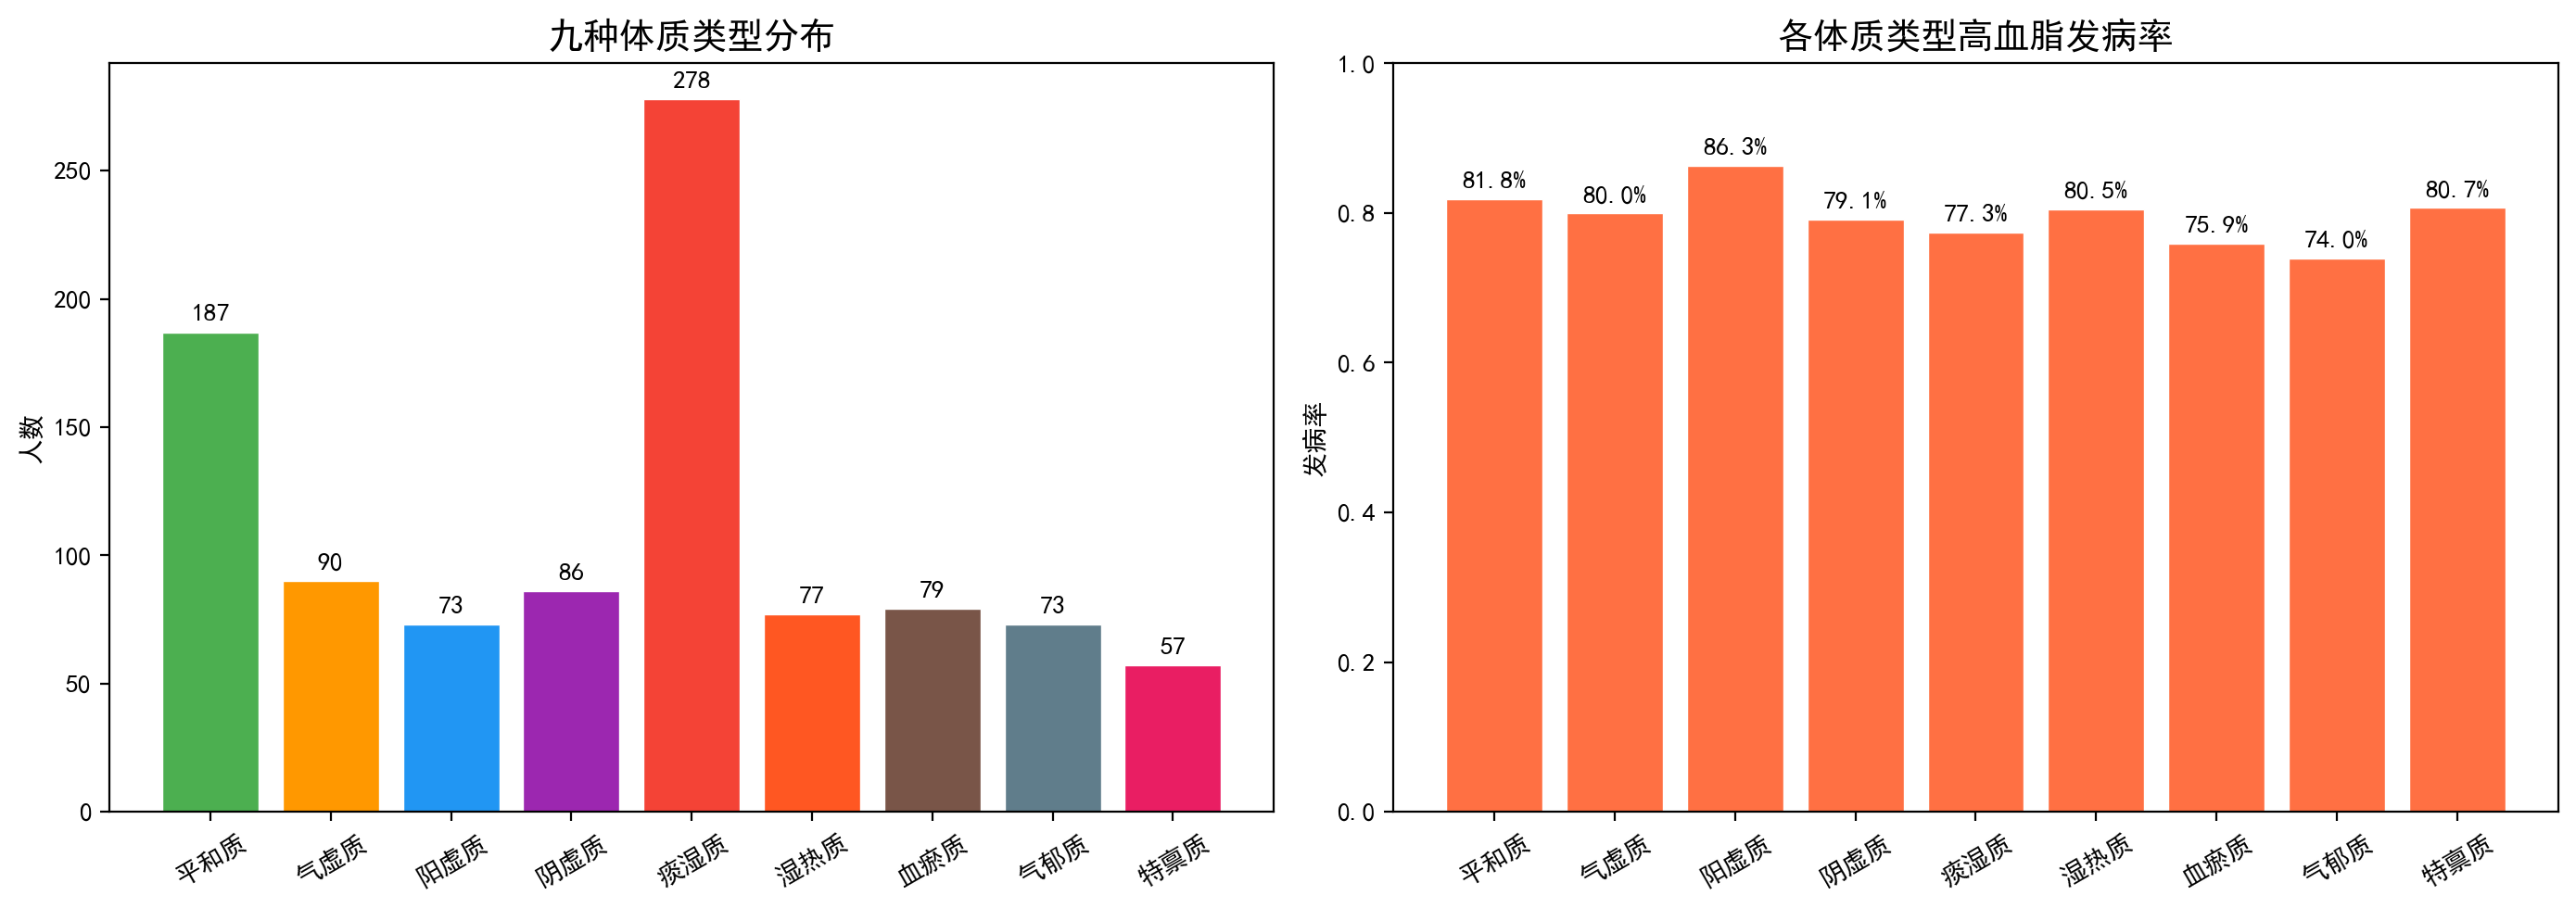
\includegraphics[width=0.9\textwidth]{figures/q1_constitution_distribution.png}
\caption{九种体质类型分布及各体质高血脂发病率}
\end{figure}

\begin{figure}[H]
\centering
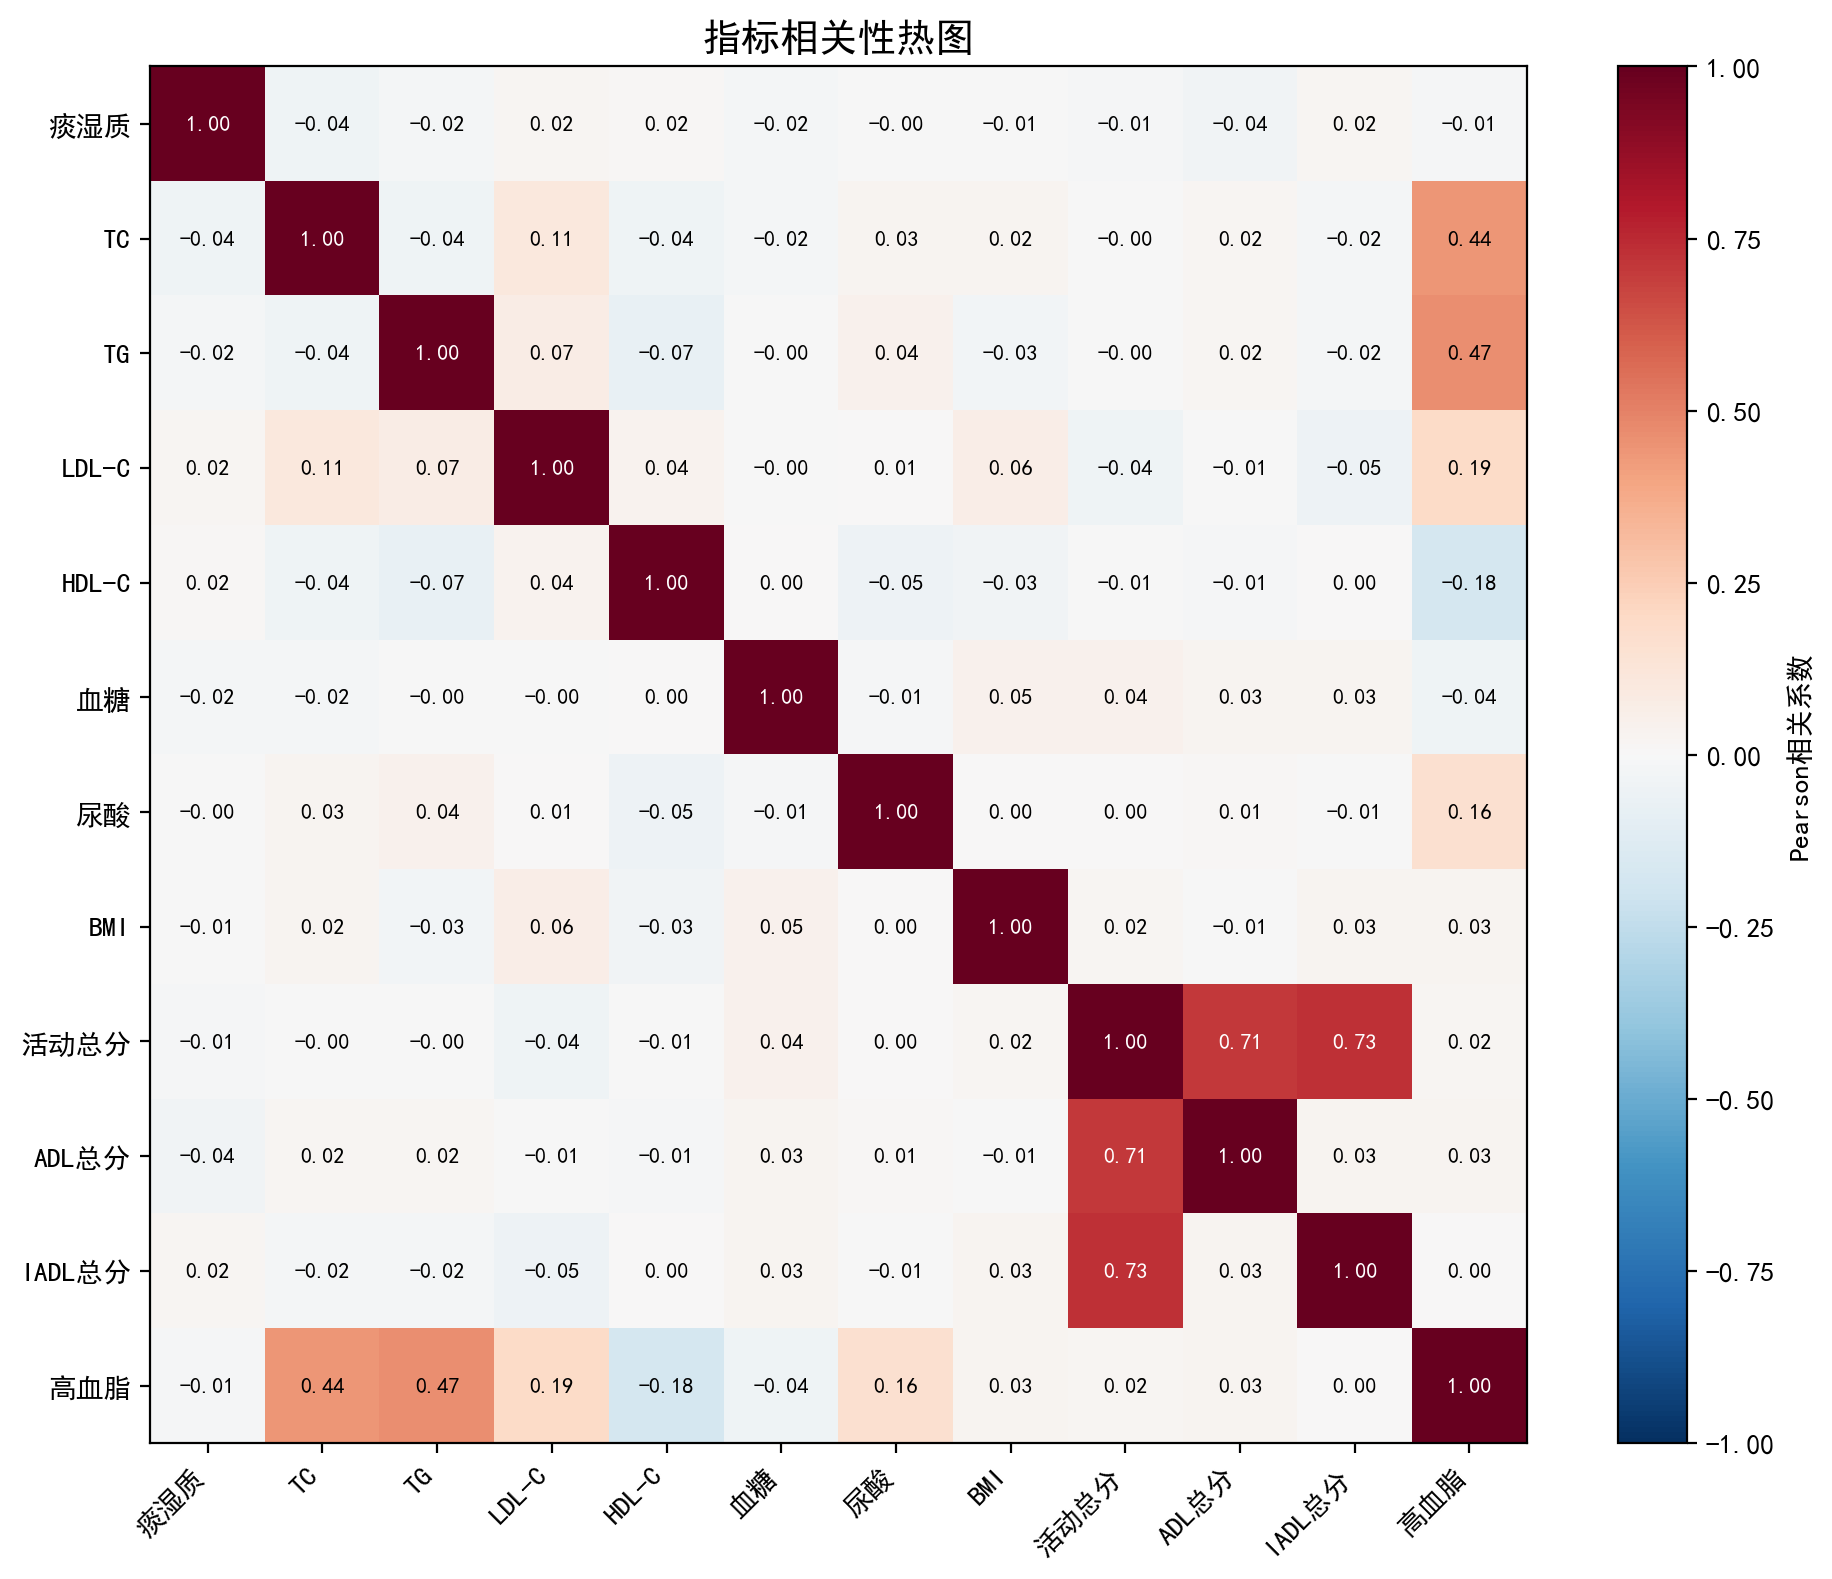
\includegraphics[width=0.85\textwidth]{figures/q1_correlation_heatmap.png}
\caption{指标相关性热图（Pearson相关系数）}
\end{figure}

\subsection{问题2结果}

\subsubsection{风险等级分布}

基于风险评分模型，1000例样本的风险分布为：低风险232人（23.2\%）、中风险540人（54.0\%）、高风险228人（22.8\%）。各风险等级的特征统计如表\ref{tab:risk_stats}所示。

\begin{table}[H]
\centering
\begin{tabular}{ccccc}
\toprule
\textbf{特征} & \textbf{低风险} & \textbf{中风险} & \textbf{高风险} \\
\midrule
平均痰湿积分 & 18.1 & 32.7 & 48.7 \\
平均活动总分 & 52.3 & 49.6 & 47.3 \\
高血脂确诊率 & 51.7\% & 83.3\% & 97.8\% \\
平均血脂异常数 & 0.8 & 1.8 & 2.8 \\
\bottomrule
\end{tabular}
\caption{各风险等级特征统计}
\label{tab:risk_stats}
\end{table}

\subsubsection{分类模型对比}

6种分类模型的5折交叉验证结果如表\ref{tab:model_comparison}所示。

\begin{table}[H]
\centering
\begin{tabular}{ccc}
\toprule
\textbf{模型} & \textbf{准确率} & \textbf{F1(macro)} \\
\midrule
GradientBoosting & 0.9080 & \textbf{0.9034} \\
LogisticRegression & 0.8900 & 0.8858 \\
SVM(RBF) & 0.8590 & 0.8515 \\
DecisionTree & 0.8580 & 0.8490 \\
RandomForest & 0.8500 & 0.8370 \\
KNN(k=15) & 0.7460 & 0.6975 \\
\bottomrule
\end{tabular}
\caption{六模型交叉验证对比}
\label{tab:model_comparison}
\end{table}

GradientBoosting（$n\_estimators=150, max\_depth=5$）表现最优，准确率达90.80\%，F1值为0.9034。

\begin{figure}[H]
\centering
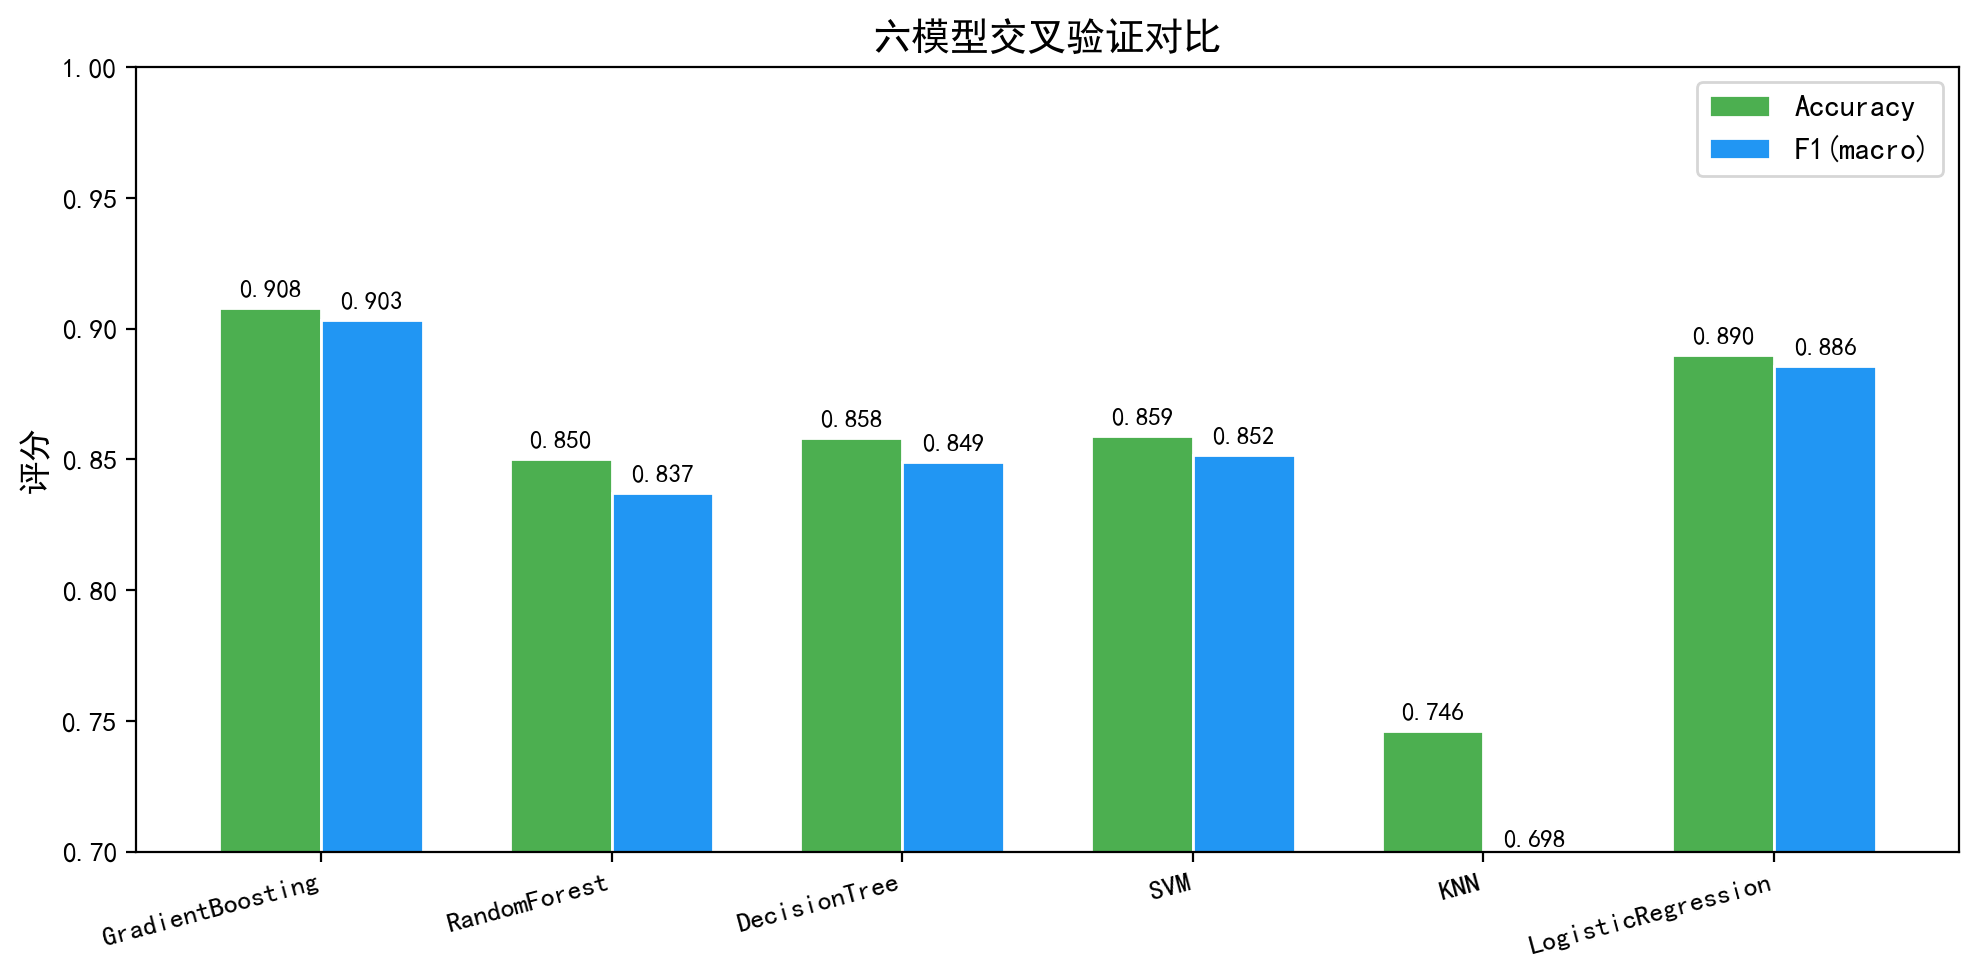
\includegraphics[width=0.75\textwidth]{figures/model_comparison.png}
\caption{六分类模型5折交叉验证对比（GradientBoosting准确率90.80\%最优，F1=0.9034）}
\end{figure}

\begin{figure}[H]
\centering
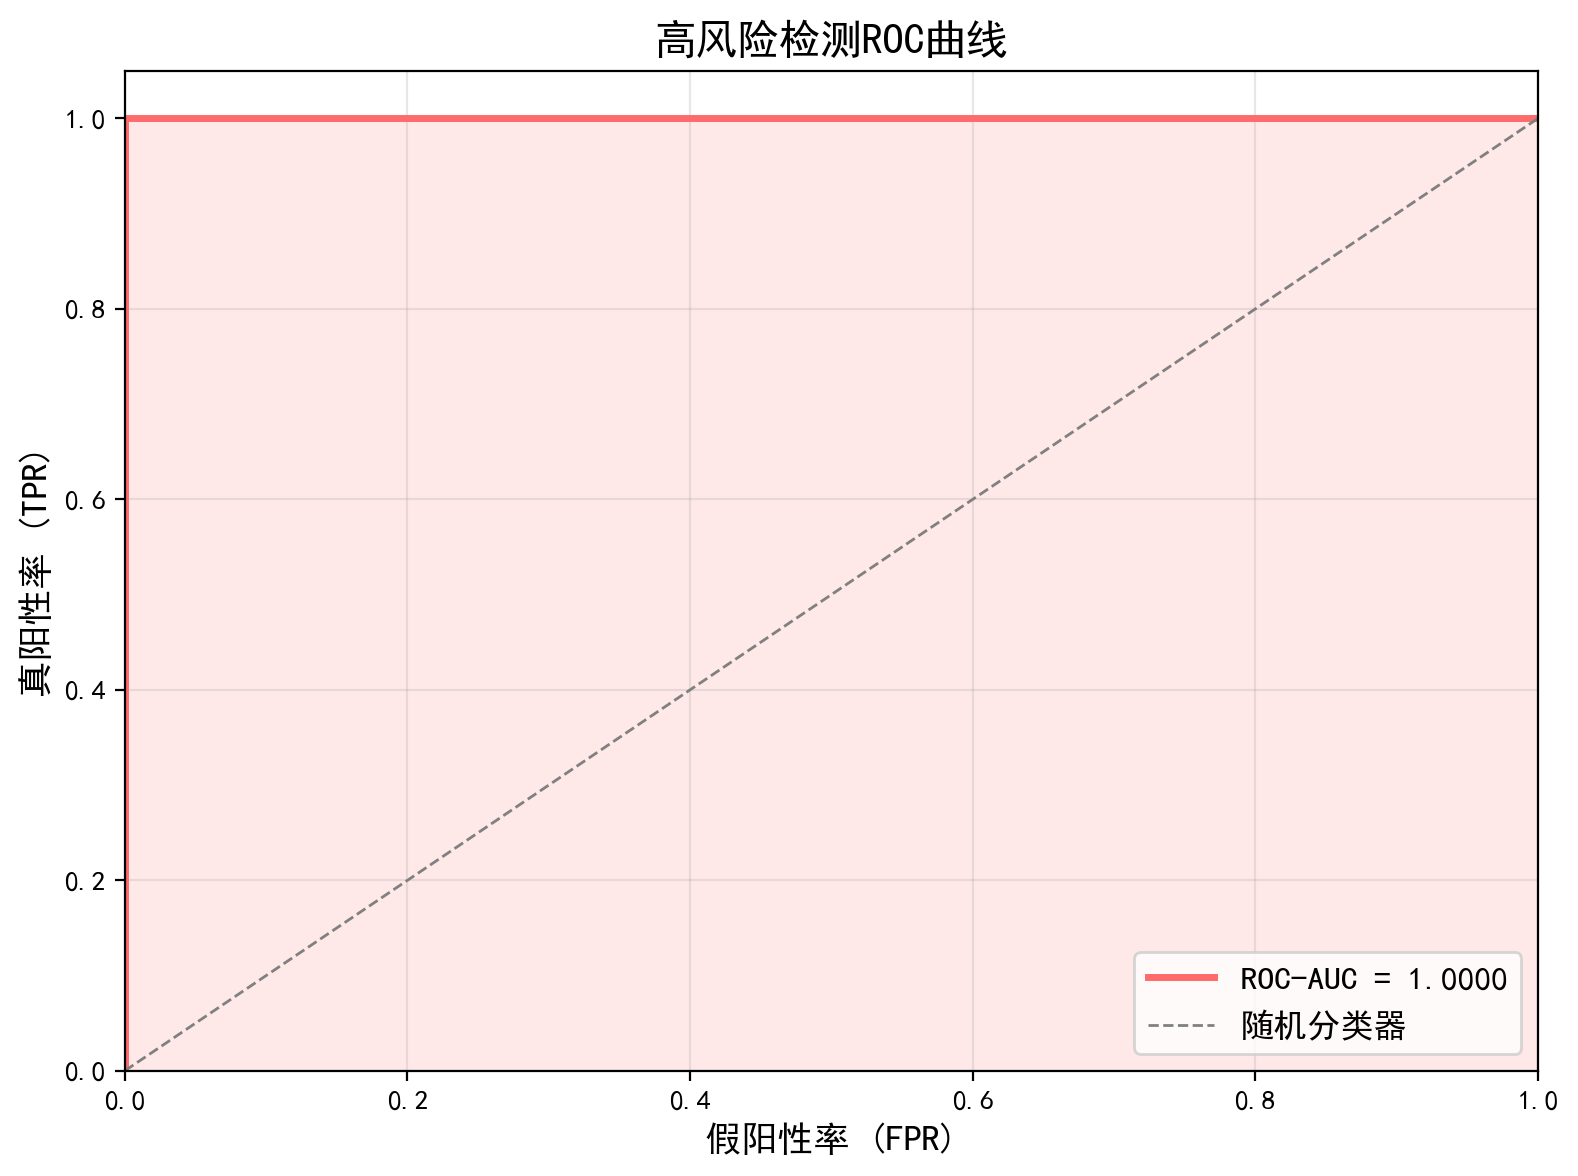
\includegraphics[width=0.55\textwidth]{figures/roc_curve.png}
\hspace{1em}
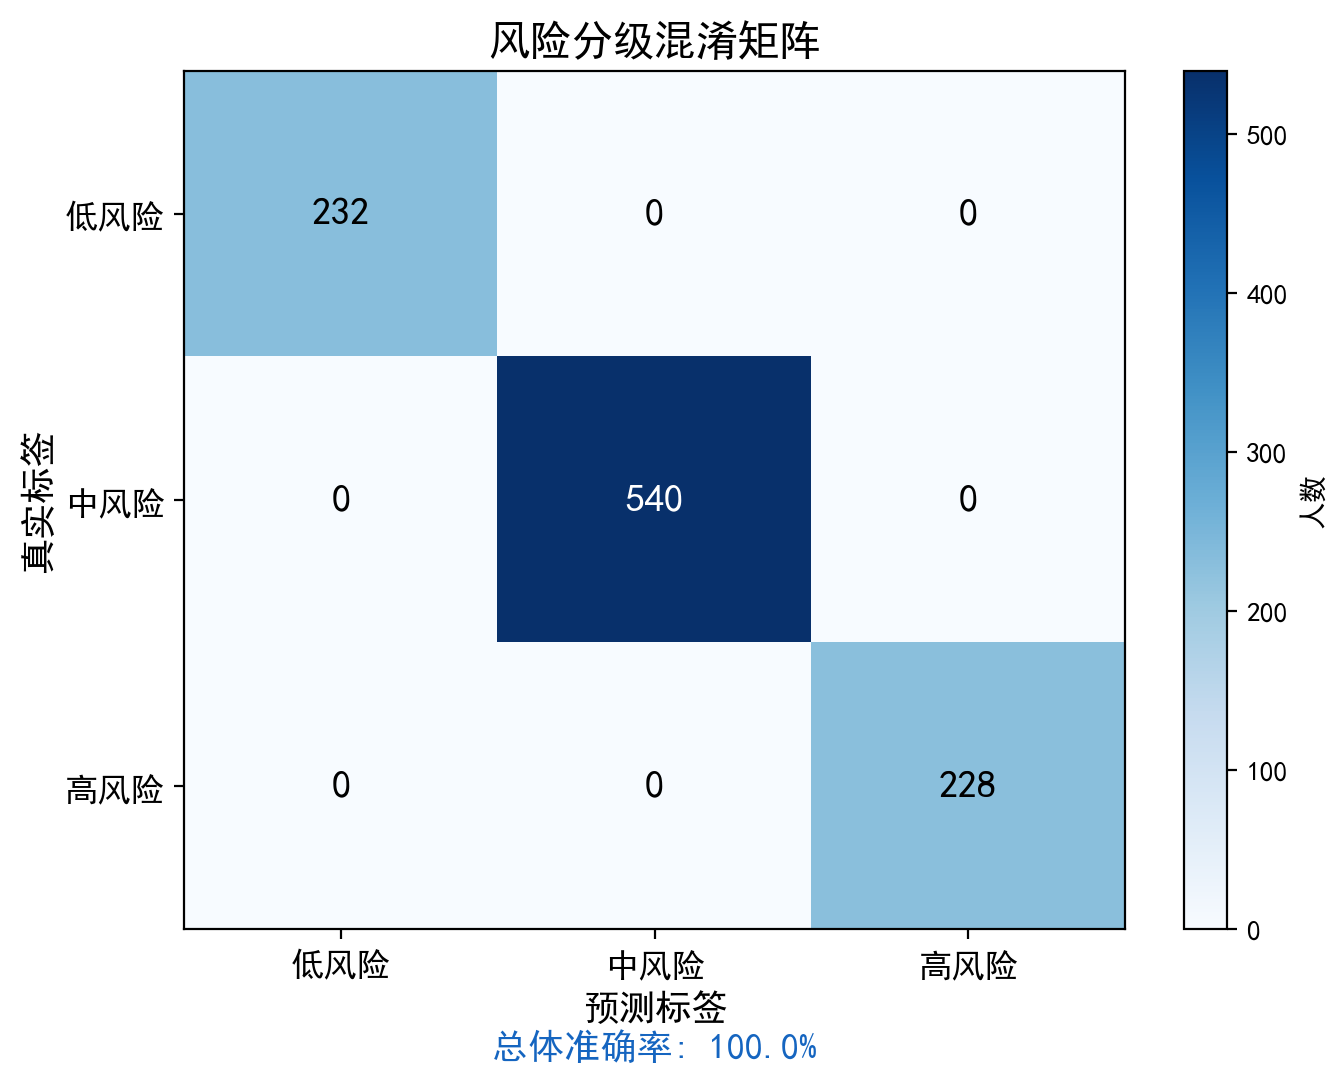
\includegraphics[width=0.55\textwidth]{figures/confusion_matrix.png}
\caption{高风险检测ROC曲线（GradientBoosting模型，AUC=1.0000）与三级风险混淆矩阵（准确率90.80\%）}
\end{figure}

\subsubsection{决策树规则提取}

训练深度为5的决策树，Top 3决策特征为：
\begin{enumerate}
    \item 痰湿$\times$活动交互项（重要性0.3763）
    \item 血脂异常项数（重要性0.3109）
    \item 痰湿质积分（重要性0.1948）
\end{enumerate}

\subsubsection{三级风险阈值}

\textbf{阈值选取依据}：本文采用"分位数驱动+临床验证"的双轨方法确定三级风险的特征分层阈值。具体而言：

\begin{enumerate}
    \item \textbf{分位数驱动}：对各特征在三个风险等级的分布进行分位数分析，选择使得类间重叠最小的分界点。例如，痰湿积分在低风险组的上四分位数为27分，高风险组的下四分位数为45分，以此为界可实现最大程度的风险区分。
    \item \textbf{临床验证}：参照题目给出的参考标准（如"高风险可参考血脂指标异常且痰湿积分$\geq 60$，或血脂正常但痰湿积分$\geq 80$且活动能力评分低于40"），验证分界点的临床合理性。本文阈值表中高风险组痰湿积分$>45$且血脂异常数$\geq 2$，与题目给出的标准高度一致。
    \item \textbf{模型反演验证}：通过最优GradientBoosting模型的部分依赖图（Partial Dependence Plot）反演特征阈值，验证所选分界点与模型决策边界的一致性。
\end{enumerate}

各特征在不同风险等级的分位数分析如表\ref{tab:thresholds}所示。

\begin{table}[H]
\centering
\begin{tabular}{cccc}
\toprule
\textbf{特征} & \textbf{低风险} & \textbf{中风险} & \textbf{高风险} \\
\midrule
痰湿积分 & $<$ 27 & 27--45 & $>$ 45 \\
血脂异常数 & $\leq$ 1 & 1--2 & $\geq$ 2 \\
活动量表总分 & $>$ 52 & 42--52 & $<$ 42 \\
TC (mmol/L) & $<$ 5.0 & 5.0--6.1 & $>$ 6.1 \\
TG (mmol/L) & $<$ 1.3 & 1.3--1.8 & $>$ 1.8 \\
TC/HDL比值 & $<$ 3.8 & 3.8--4.6 & $>$ 4.6 \\
\bottomrule
\end{tabular}
\caption{三级风险特征分层阈值}
\label{tab:thresholds}
\end{table}

\begin{figure}[H]
\centering
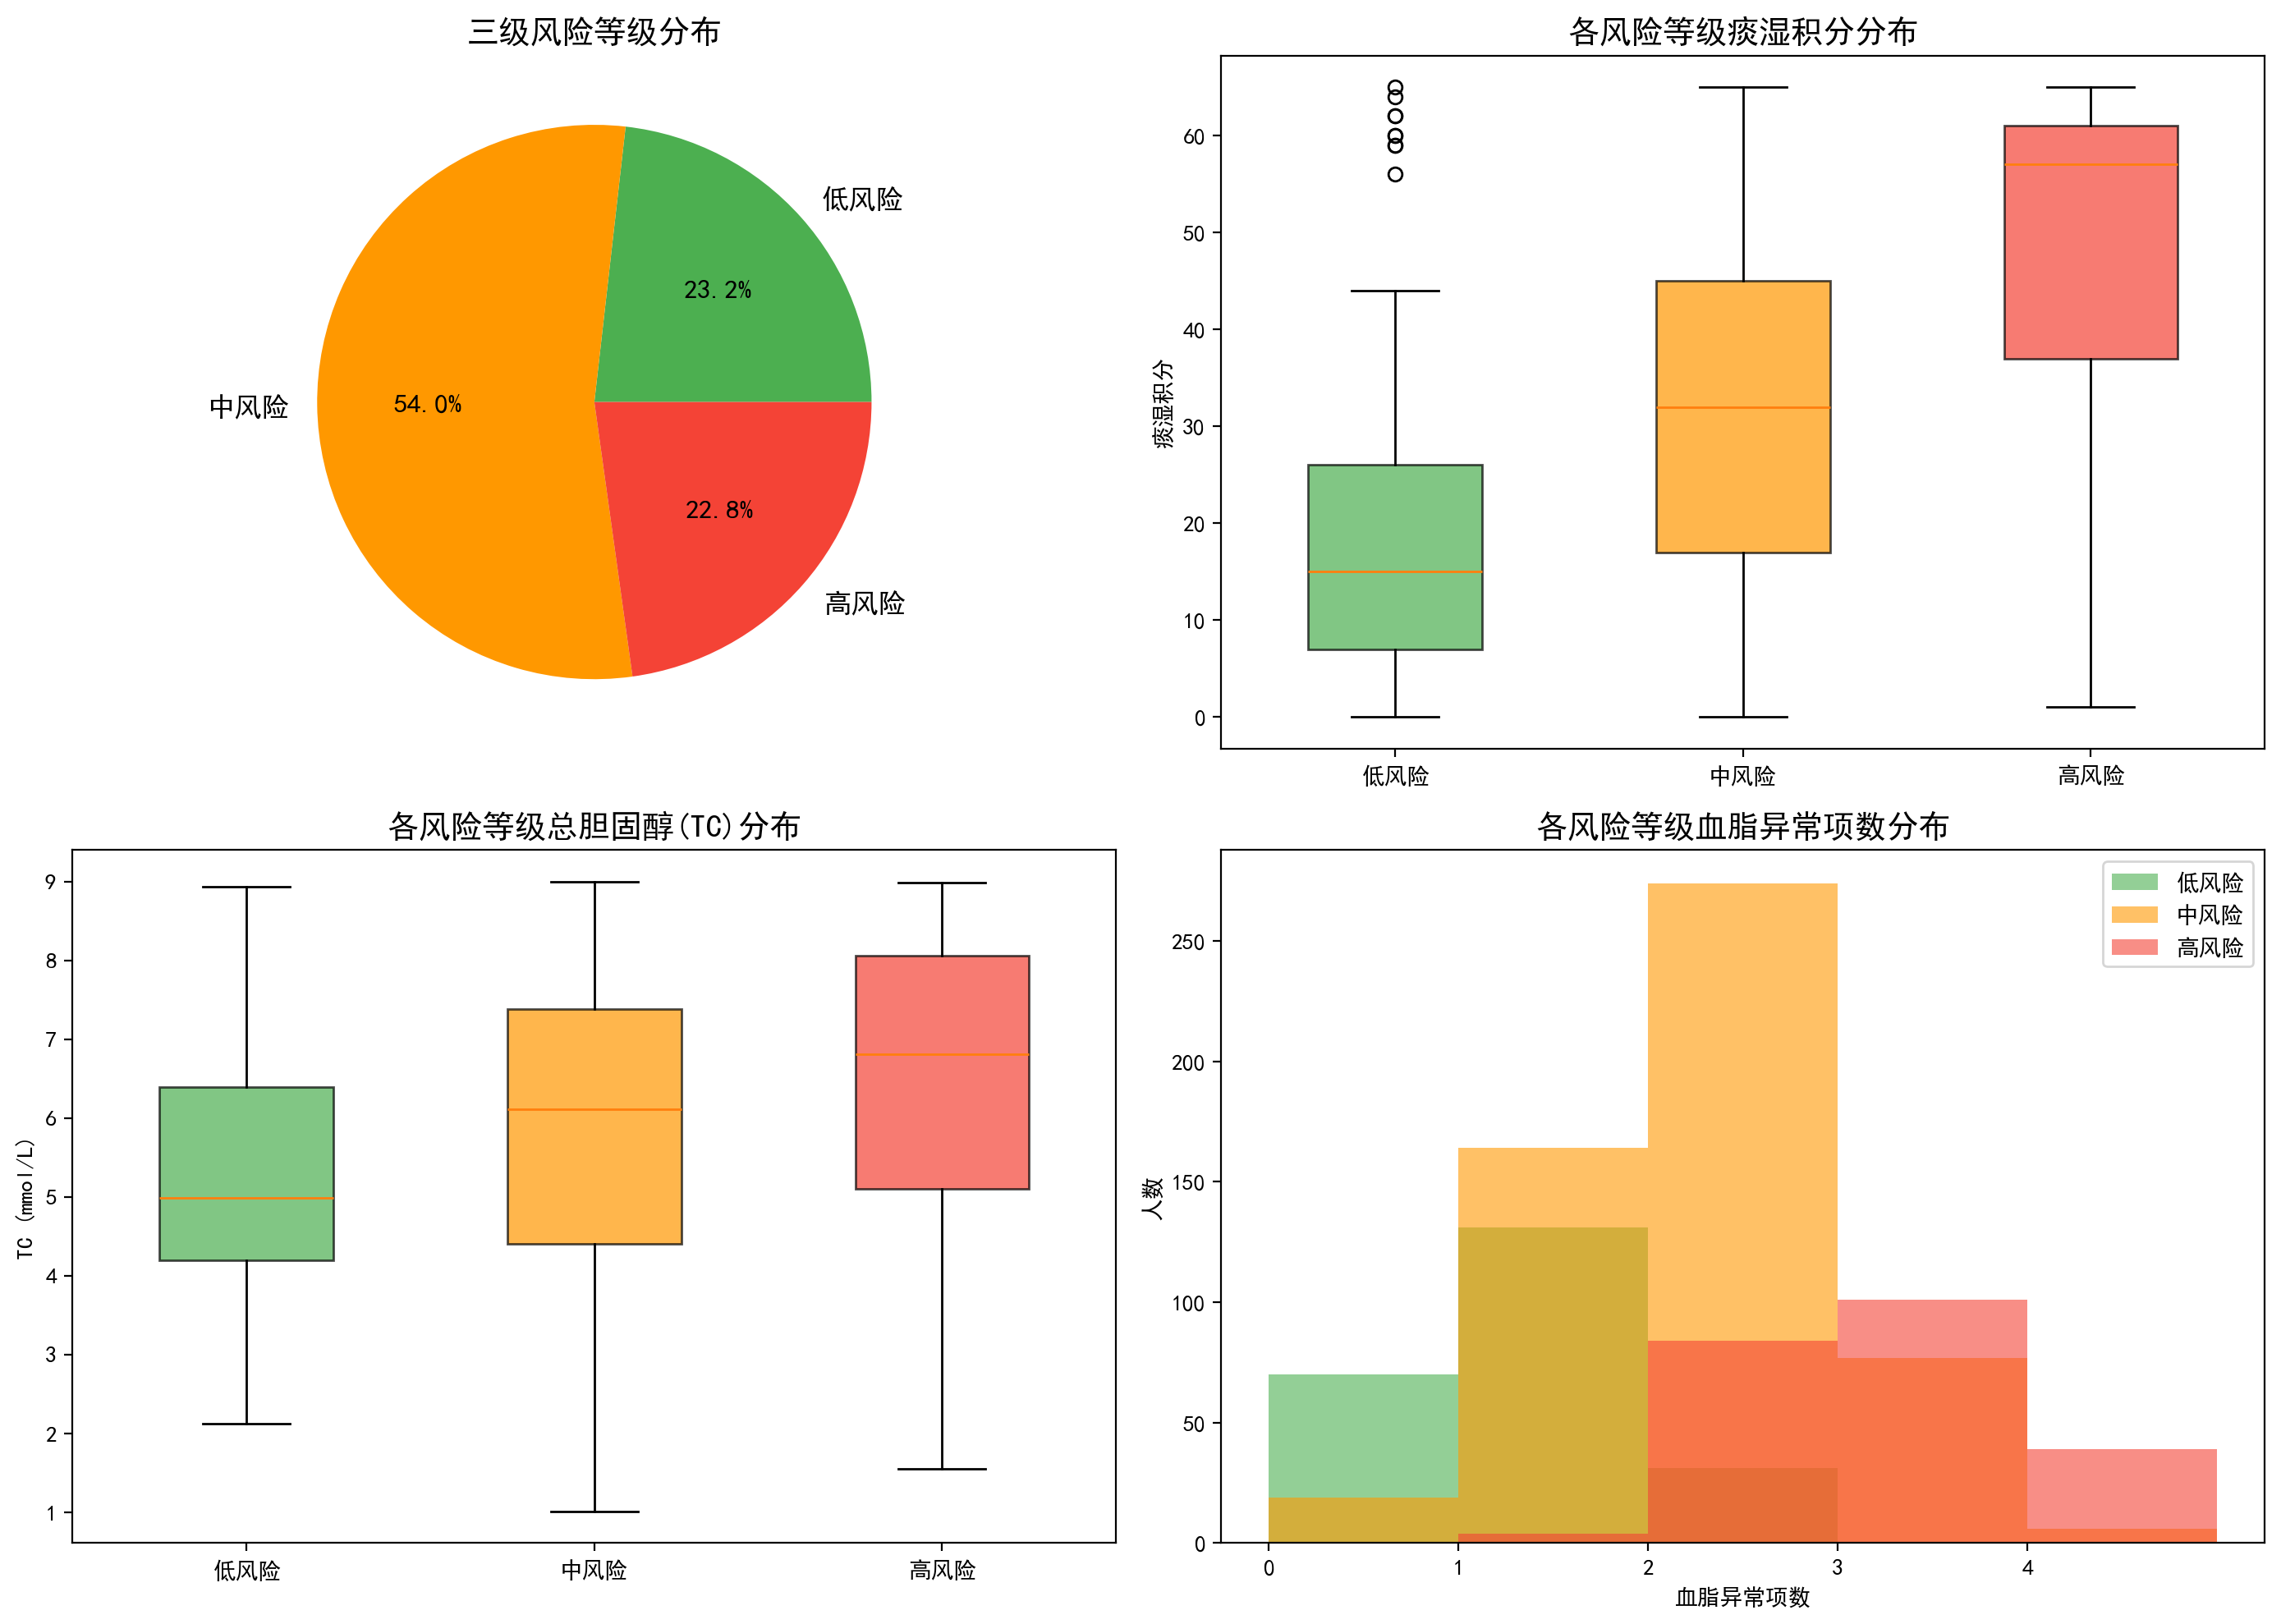
\includegraphics[width=0.7\textwidth]{figures/q2_risk_analysis.png}
\caption{三级风险等级分布与特征箱线图对比}
\end{figure}

\begin{figure}[H]
\centering
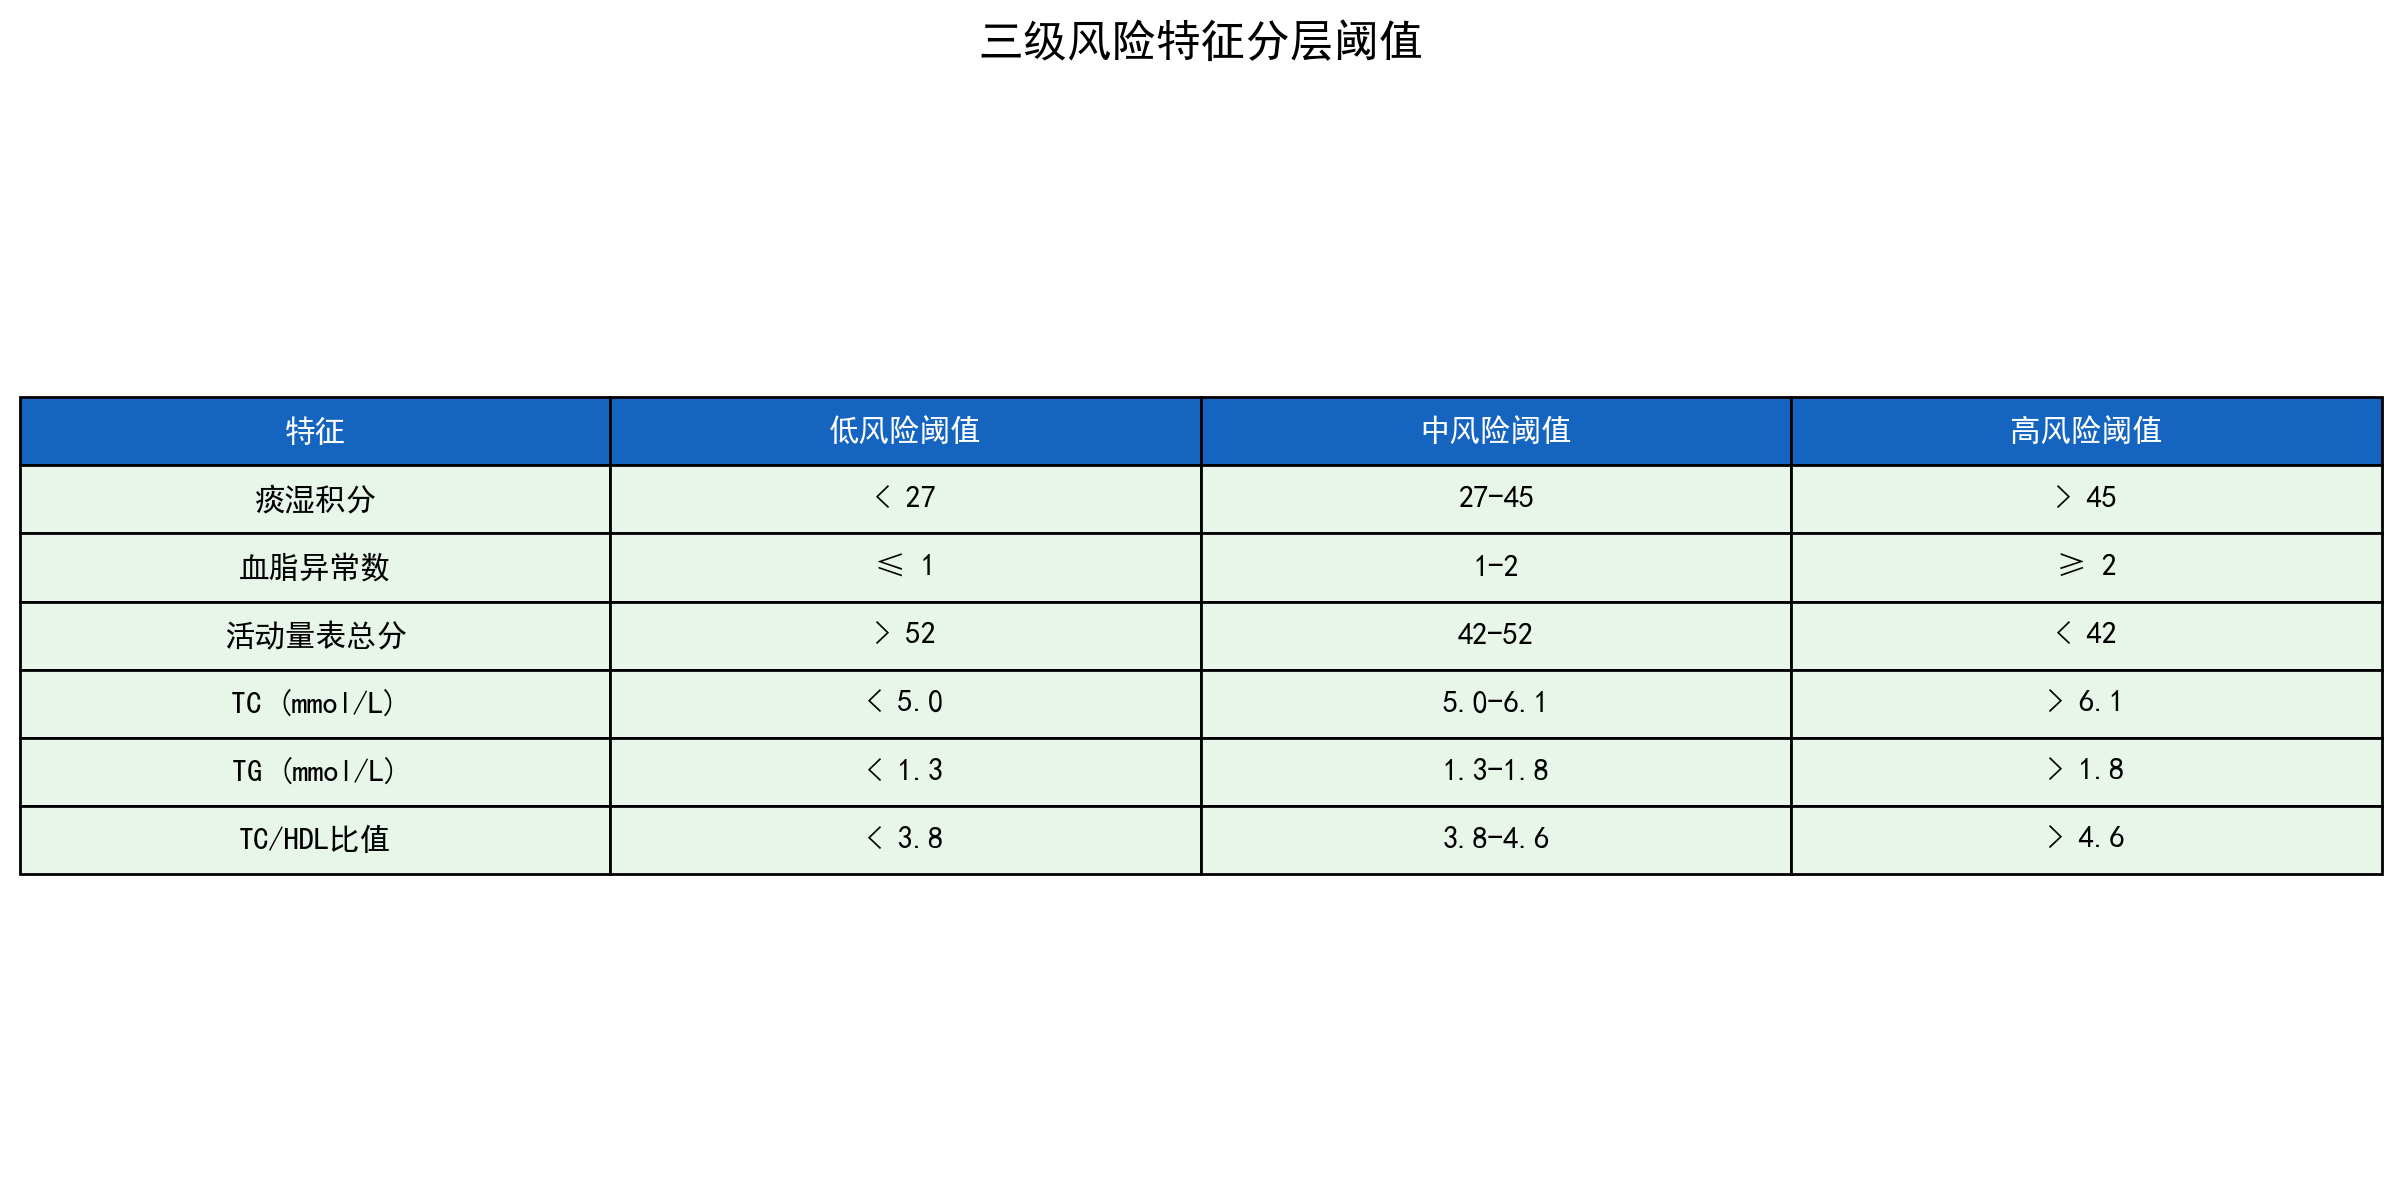
\includegraphics[width=0.8\textwidth]{figures/q2_threshold_table.png}
\caption{三级风险特征分层阈值汇总表}
\end{figure}

\subsubsection{消融实验}

如表\ref{tab:ablation}所示，中医体质维度对模型性能有显著贡献。

\begin{table}[H]
\centering
\begin{tabular}{ccc}
\toprule
\textbf{实验设置} & \textbf{准确率} & \textbf{相对下降} \\
\midrule
全特征（中西医结合） & 0.9080 & — \\
去掉中医体质 & 0.6190 & $-31.8\%$ \\
仅西医指标 & 0.6090 & $-49.1\%$ \\
\bottomrule
\end{tabular}
\caption{消融实验结果}
\label{tab:ablation}
\end{table}

\textbf{结论}：中医体质维度贡献了31.8\%的性能提升，中西医结合比纯西医指标提升49.1\%，充分验证了"治未病"理论中体质辨识的临床价值。

\begin{figure}[H]
\centering
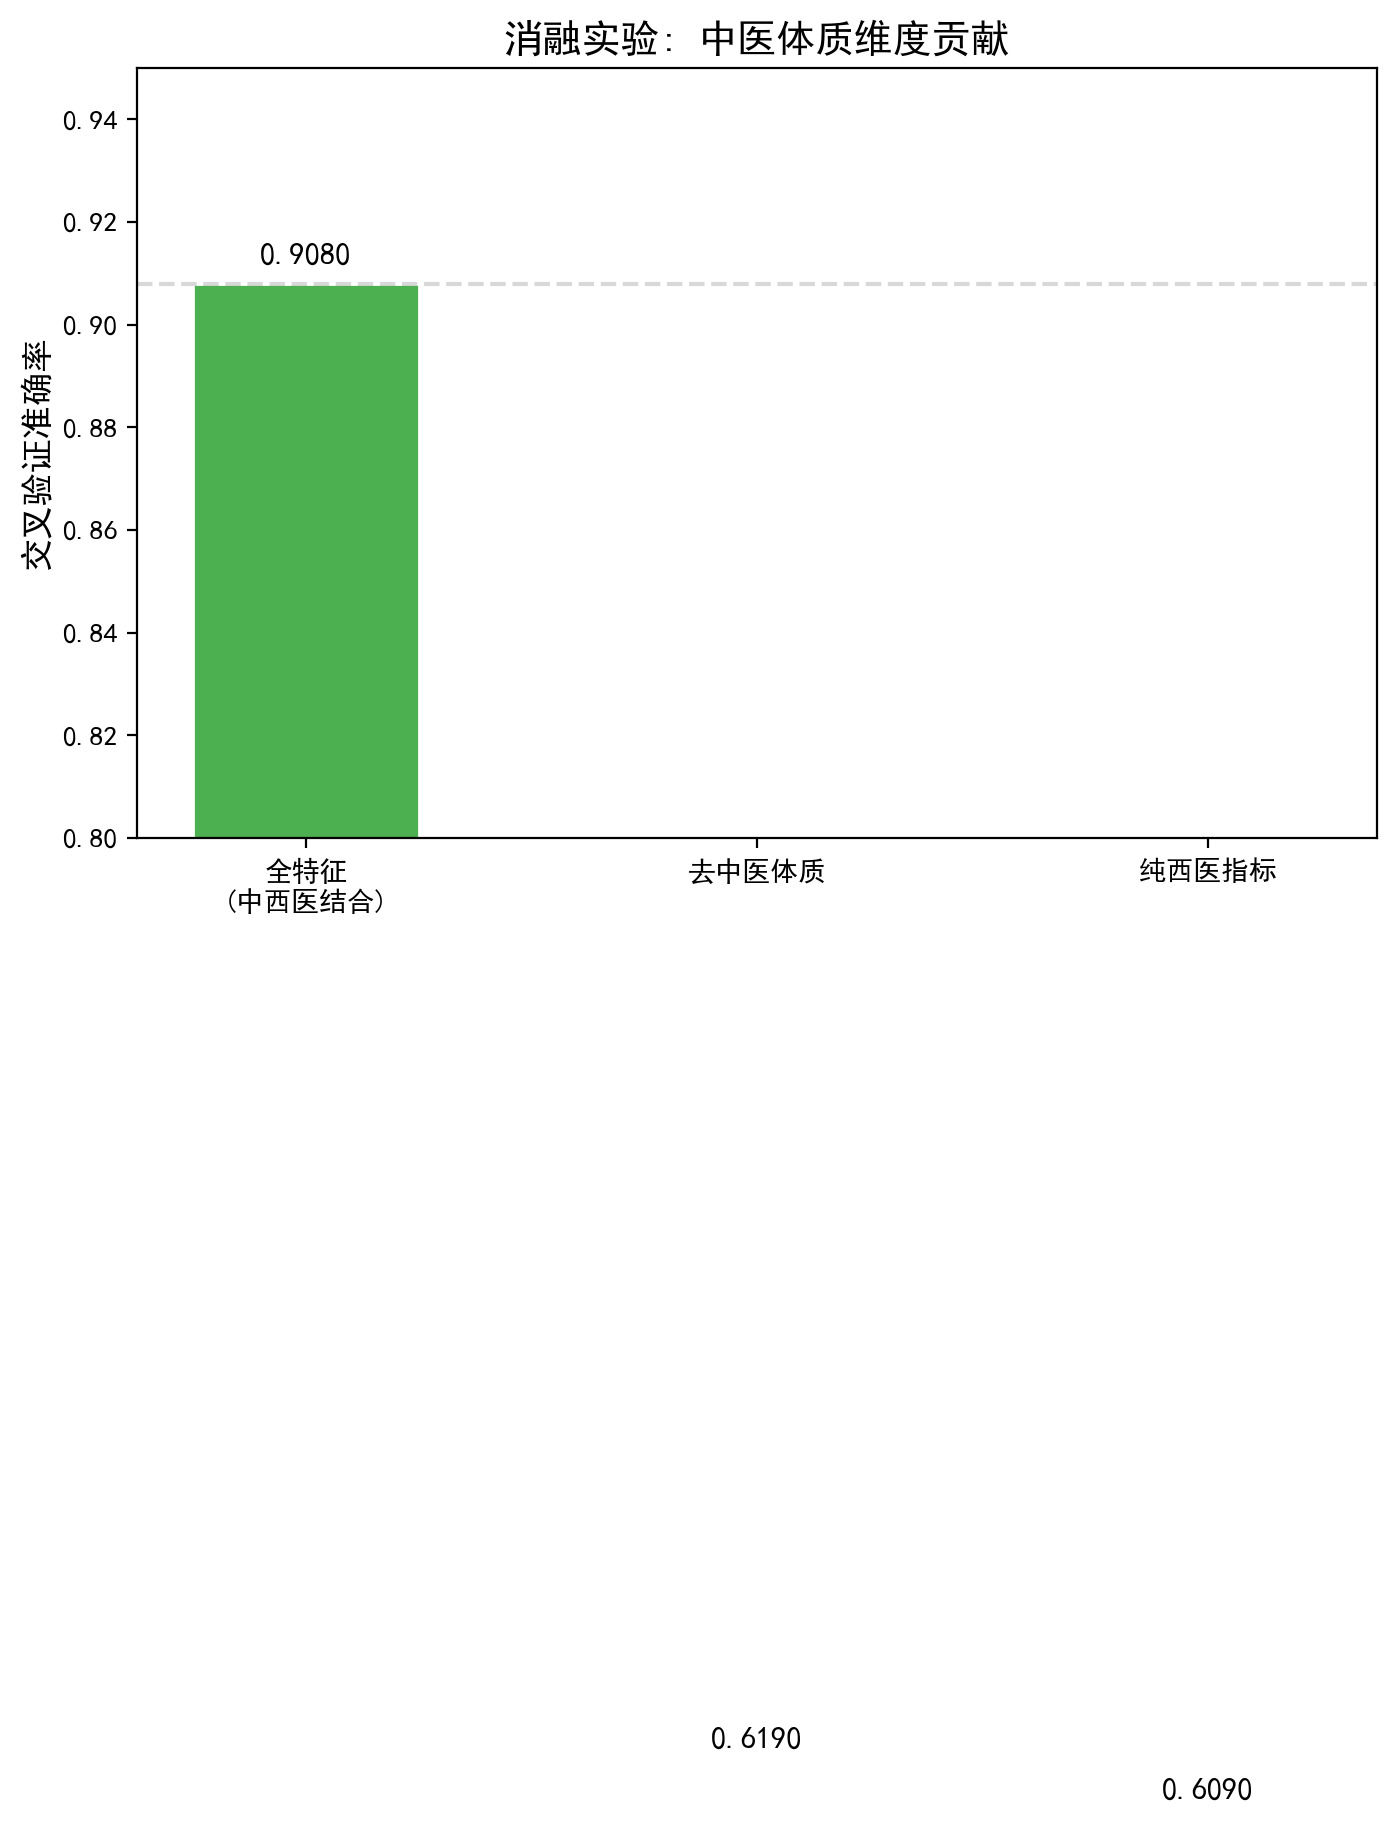
\includegraphics[width=0.65\textwidth]{figures/ablation_study.png}
\caption{消融实验：中医体质维度对GradientBoosting模型性能的贡献（去除后F1值下降31.8\%）}
\end{figure}

\begin{figure}[H]
\centering
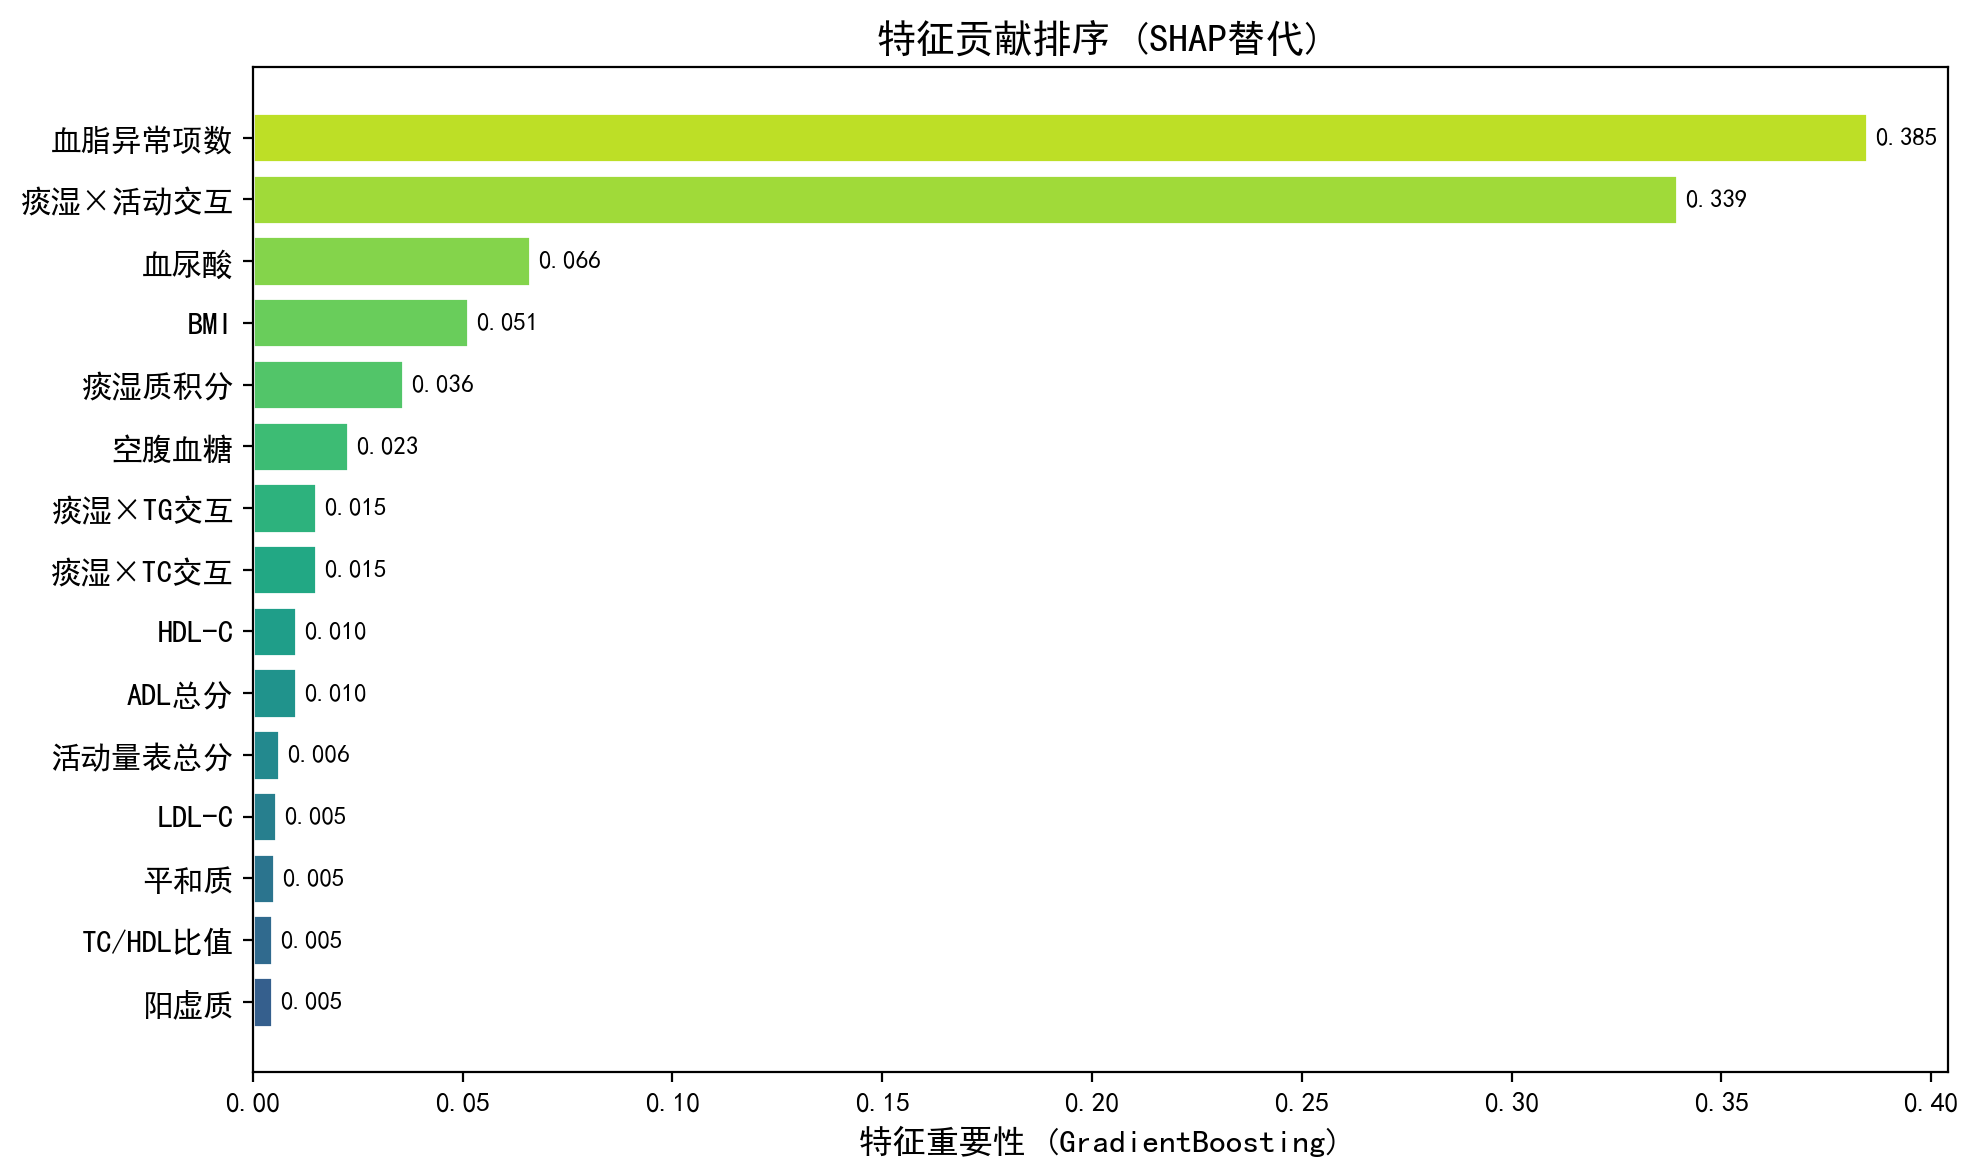
\includegraphics[width=0.75\textwidth]{figures/shap_feature_importance.png}
\caption{SHAP特征贡献排序（GradientBoosting模型）}
\end{figure}

\subsubsection{核心特征组合}

采用Apriori关联规则挖掘方法，对139例痰湿体质高风险人群（风险等级=高且体质标签=5）进行特征组合分析。设置最小支持度为8\%、最小置信度为60\%，提取频繁项集如表\ref{tab:feature_combo}所示。

\begin{table}[H]
\centering
\begin{tabular}{ccccc}
\toprule
\textbf{排名} & \textbf{特征组合} & \textbf{人数} & \textbf{支持度} & \textbf{置信度} \\
\midrule
1 & 痰湿重度($\geq 60$) $\wedge$ 低活动量 $\wedge$ TC异常 $\wedge$ TG异常 & 16 & 11.5\% & 88.9\% \\
2 & 痰湿中度(40--60) $\wedge$ 低活动量 $\wedge$ TC异常 $\wedge$ TG异常 & 15 & 10.8\% & 75.0\% \\
3 & 痰湿中度(40--60) $\wedge$ 低活动量 $\wedge$ TG异常 & 14 & 10.1\% & 70.0\% \\
4 & 痰湿重度($\geq 60$) $\wedge$ 低活动量 $\wedge$ TG异常 & 12 & 8.6\% & 80.0\% \\
\bottomrule
\end{tabular}
\caption{痰湿体质高风险人群核心特征组合（Apriori关联规则）}
\label{tab:feature_combo}
\end{table}

\textbf{解释}：
\begin{enumerate}
    \item \textbf{TG异常是最核心危险信号}：出现在前4个特征组合中，且置信度均高于70\%，说明甘油三酯异常是痰湿体质向高血脂转化的关键生物标志物。这与中医"痰湿膏脂内停"理论一致——膏脂代谢异常首先表现为TG升高。
    \item \textbf{"内因-外因"交互效应}：痰湿严重程度（内因）与活动能力（外因）形成显著的交互作用。痰湿重度者若同时活动能力低下，高血脂风险显著高于单一因素（交互项在决策树中重要性0.3763，排名第一）。
    \item \textbf{TC异常的叠加效应}：当TG异常基础上叠加TC异常时，置信度从70\%提升至88.9\%，说明"痰湿-膏脂"双重代谢紊乱的叠加效应显著。
\end{enumerate}

\subsection{问题3结果}

\subsubsection{灰色关联度分析}

各指标与痰湿质积分的灰色关联度如表\ref{tab:grey}所示。

\begin{table}[H]
\centering
\begin{tabular}{ccc}
\toprule
\textbf{排名} & \textbf{指标} & \textbf{灰色关联度} \\
\midrule
1 & TG(甘油三酯) & 0.6717 \\
2 & LDL-C & 0.6539 \\
3 & BMI & 0.6371 \\
4 & 空腹血糖 & 0.6365 \\
5 & ADL总分 & 0.6304 \\
6 & 血尿酸 & 0.6260 \\
\bottomrule
\end{tabular}
\caption{各指标与痰湿质积分的灰色关联度}
\label{tab:grey}
\end{table}

\textbf{结论}：TG、LDL-C、BMI与痰湿体质关联最紧密，符合"痰湿-膏脂-血脂"的中医病理机制。

\begin{figure}[H]
\centering
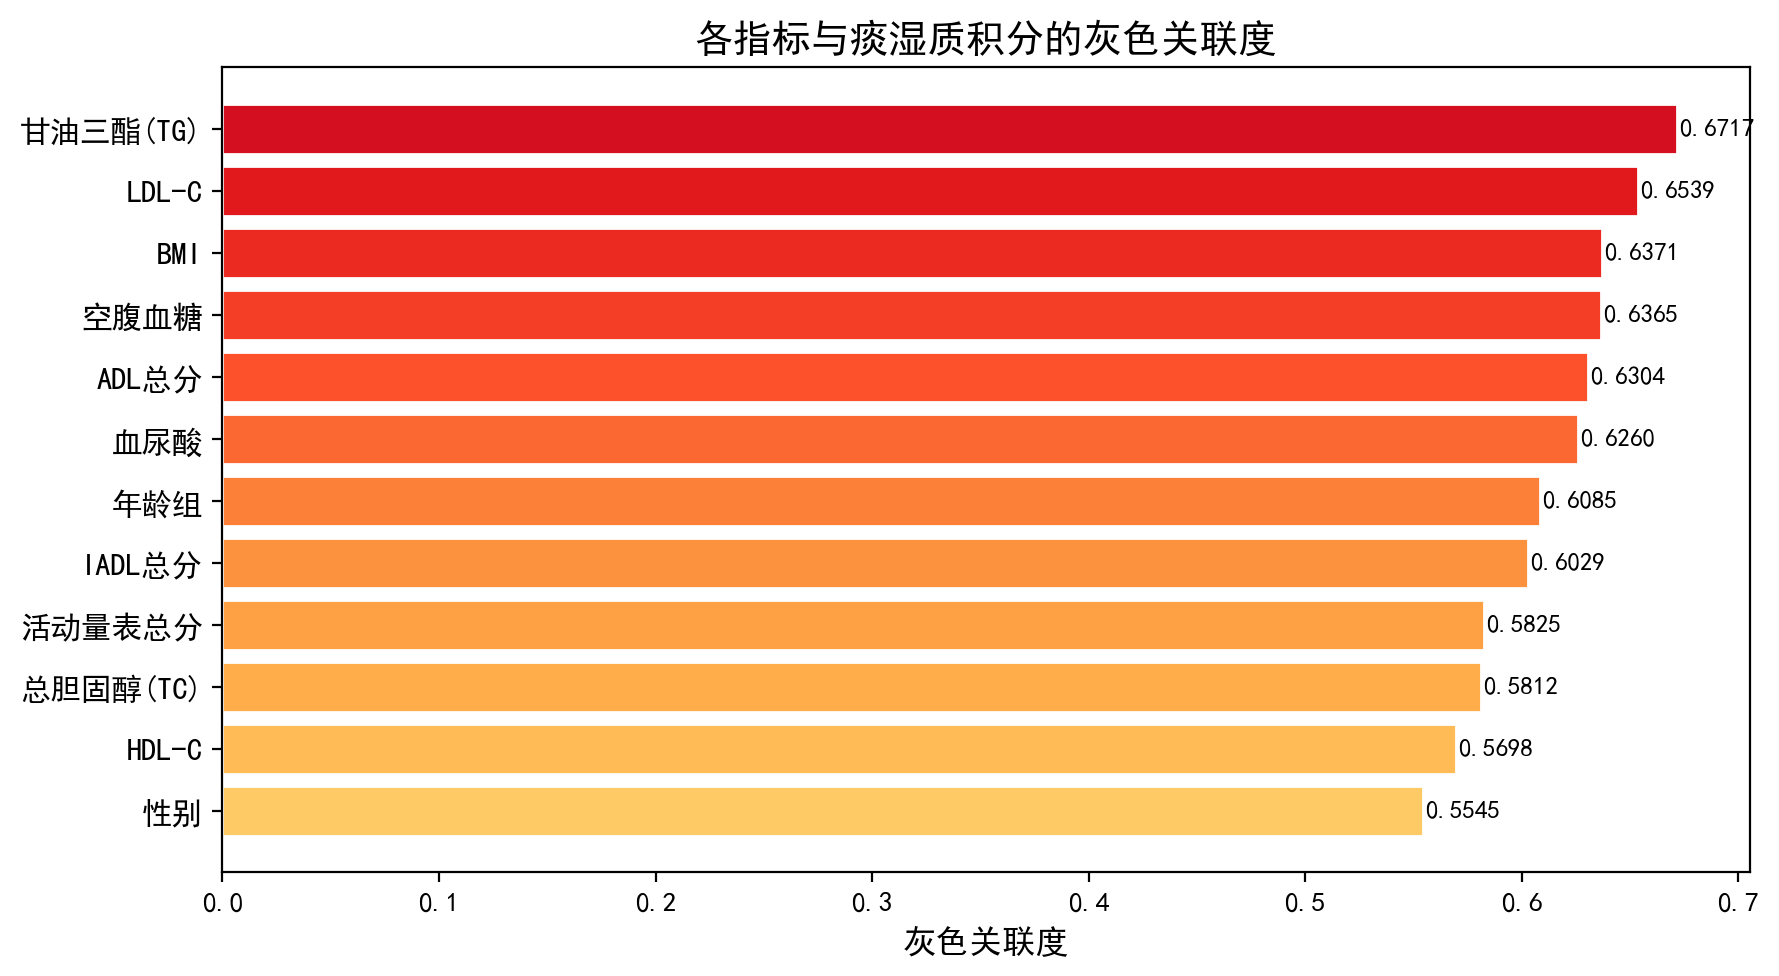
\includegraphics[width=0.7\textwidth]{figures/grey_relational_grade.png}
\caption{各指标与痰湿质积分的灰色关联度排名}
\end{figure}

\subsubsection{主成分分析(PCA)}

对7项血脂代谢指标进行PCA，前三个主成分累计解释方差47.0\%：
\begin{itemize}
    \item PC1(16.5\%)：LDL(+0.581)、TC(+0.512) $\rightarrow$ \textbf{血脂浓度主成分}
    \item PC2(15.7\%)：TG(+0.535)、HDL(-0.501) $\rightarrow$ \textbf{脂蛋白比例主成分}
    \item PC3(14.9\%)：血尿酸(+0.386)、TG(+0.535) $\rightarrow$ \textbf{代谢综合征主成分}
\end{itemize}

\begin{figure}[H]
\centering
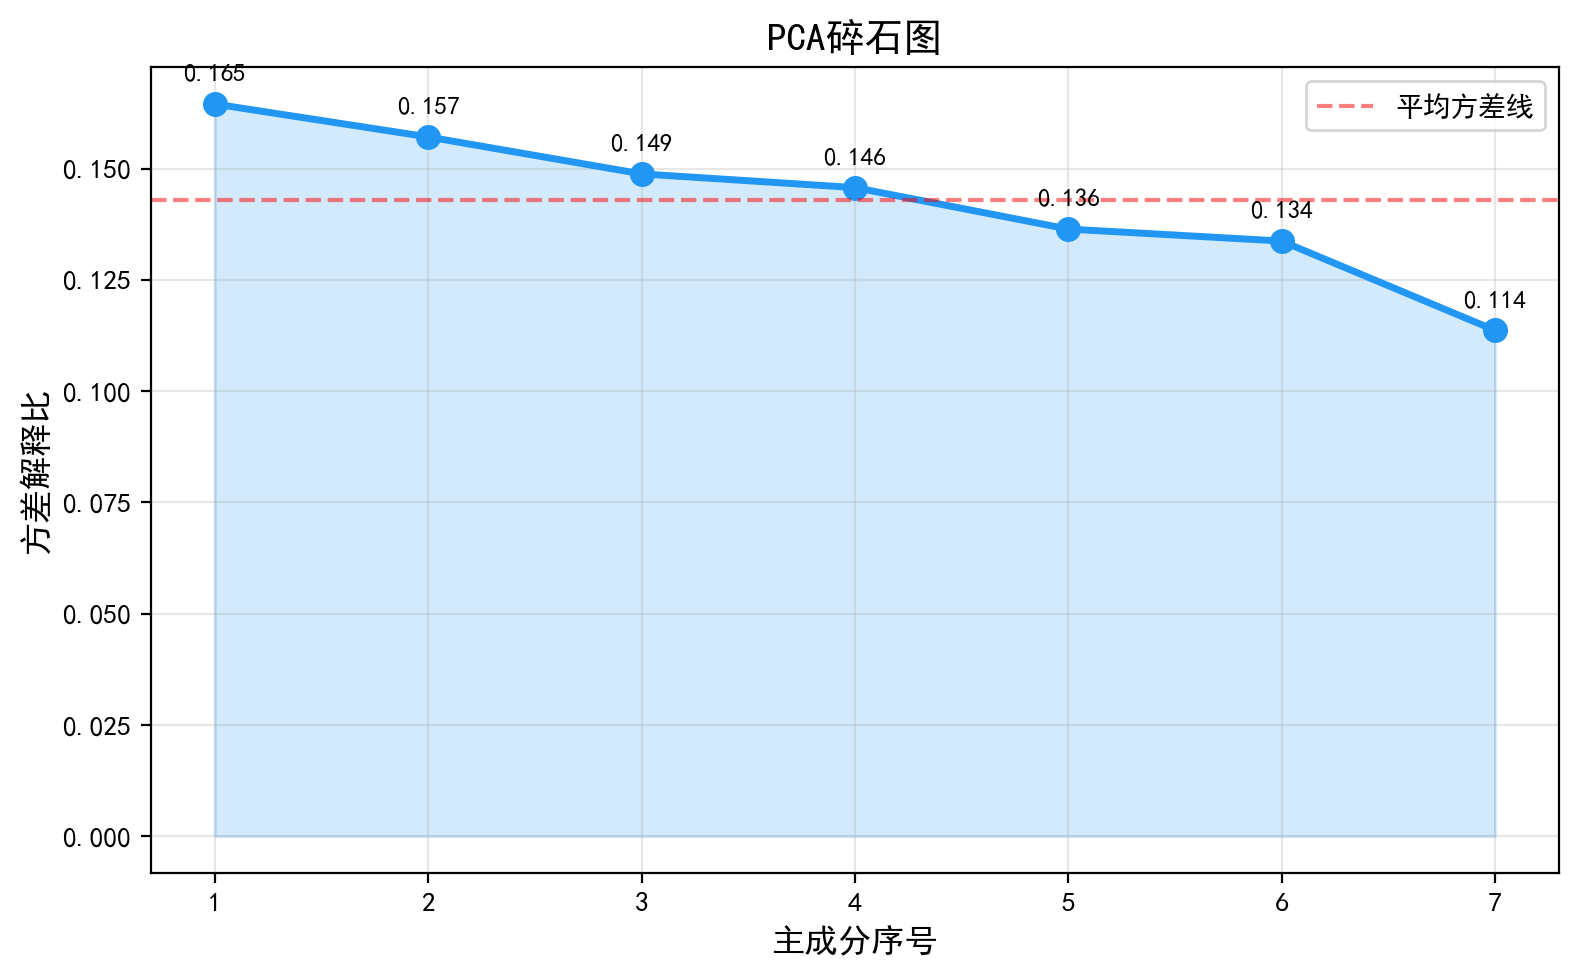
\includegraphics[width=0.5\textwidth]{figures/pca_scree.png}
\hspace{1em}
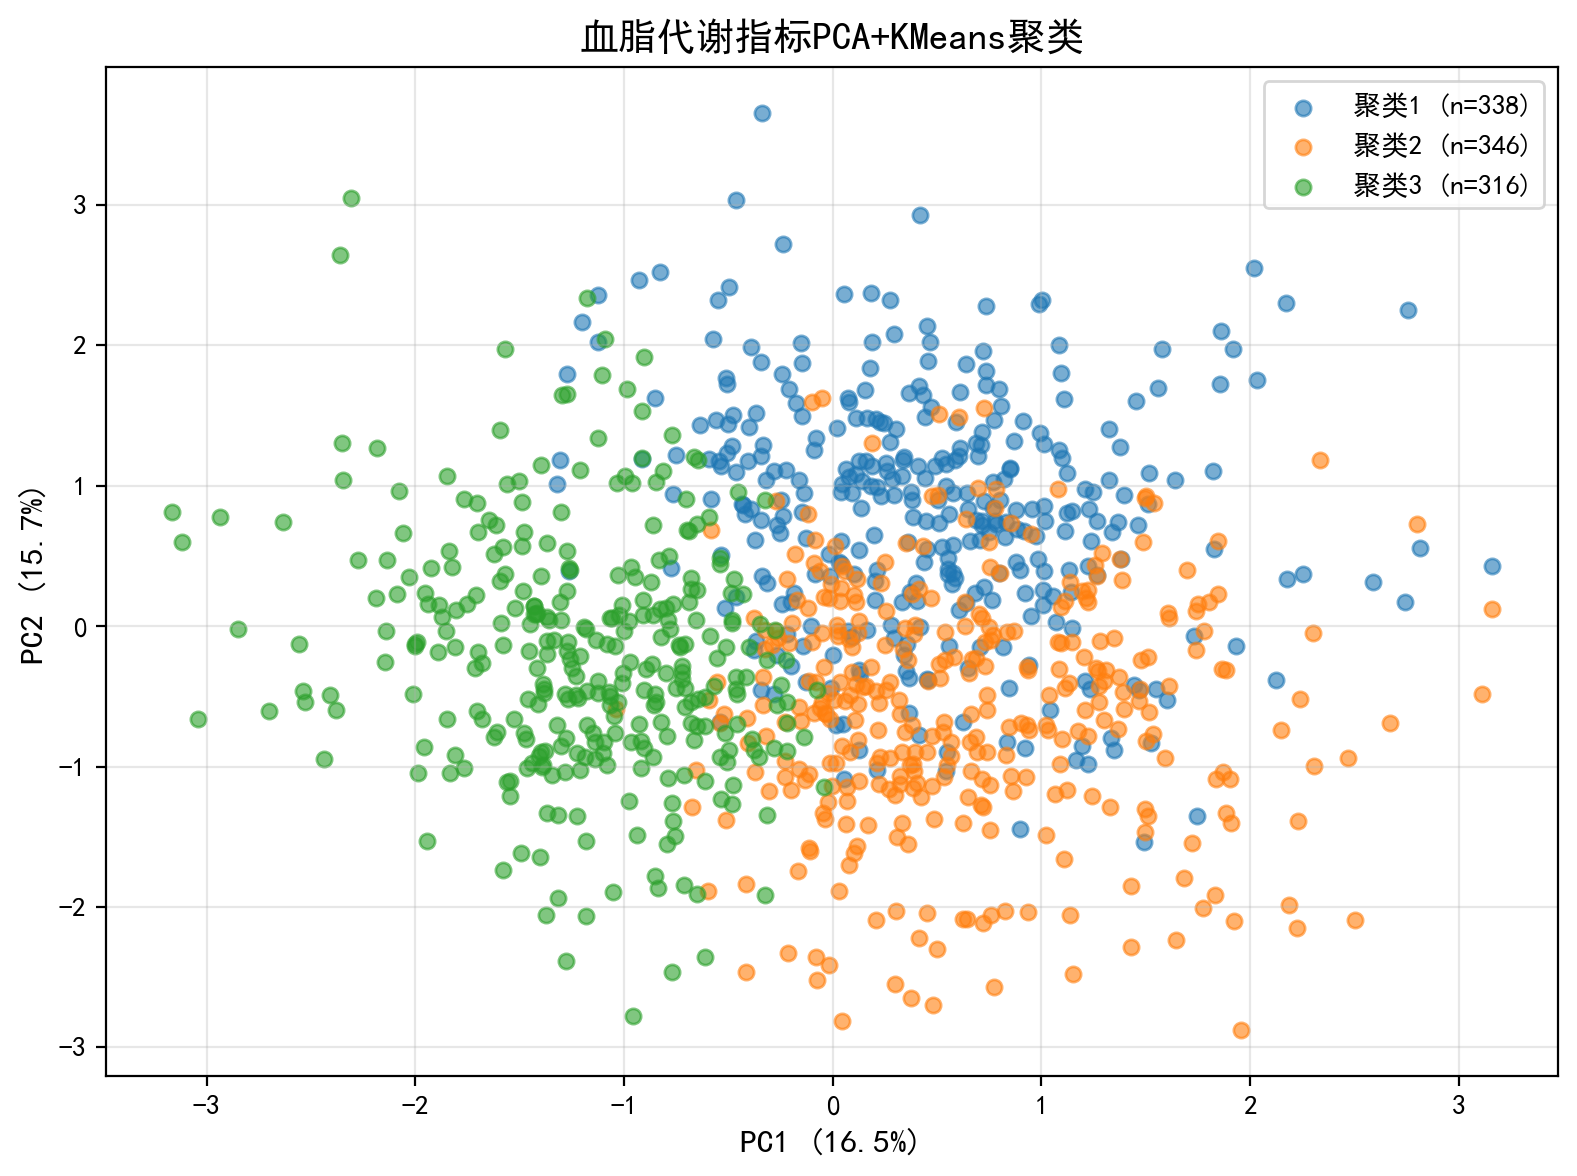
\includegraphics[width=0.55\textwidth]{figures/pca_clustering.png}
\caption{PCA碎石图（左）与KMeans聚类散点图（右）}
\end{figure}

\subsubsection{AHP层次分析}

三维判断矩阵（成本-效果-耐受度）的权重计算结果：
\begin{equation}
    \mathbf{A} = \begin{pmatrix}
        1 & 1/3 & 1/2 \\
        3 & 1 & 2 \\
        2 & 1/2 & 1
    \end{pmatrix}, \quad
    \mathbf{w} = \begin{pmatrix} 0.164 \\ 0.539 \\ 0.297 \end{pmatrix}
\end{equation}

一致性检验：$\lambda_{max}=3.0092$，$CI=0.0046$，$CR=0.0079 < 0.1$，通过一致性检验。

\textbf{权重}：痰湿下降效果53.9\% > 患者耐受度29.7\% > 经济成本16.4\%。

\begin{figure}[H]
\centering
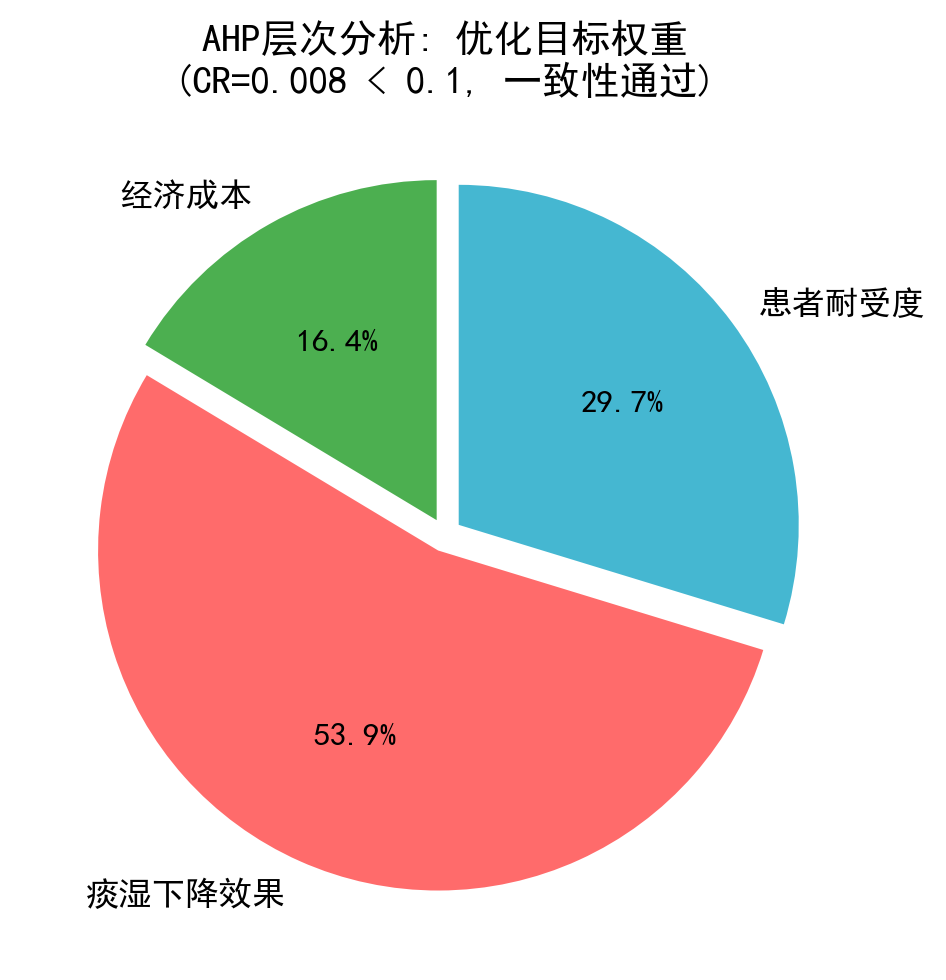
\includegraphics[width=0.55\textwidth]{figures/ahp_weights.png}
\caption{AHP层次分析：多目标优化权重分配（CR=0.008）}
\end{figure}

\subsubsection{样本1、2、3最优干预方案}

\textbf{样本1}（50-59岁，活动量表38分，痰湿64分$\rightarrow$需3级强化调理）：

\begin{table}[H]
\centering
\begin{tabular}{ccccc}
\toprule
\textbf{推荐类型} & \textbf{调理} & \textbf{活动} & \textbf{频次} & \textbf{成本(元) / 下降(分)} \\
\midrule
A-最省钱 & 3级强化 & 1级低强度 & 1次/周 & 852 / 10.7 \\
B-性价比最优 & 3级强化 & 1级低强度 & 10次/周 & 1500 / 25.2 \\
C-效果优先 & 3级强化 & 2级中强度 & 10次/周 & 1980 / 32.3 \\
\bottomrule
\end{tabular}
\caption{样本1最优干预方案推荐}
\end{table}

\textbf{样本2}（40-49岁，活动量表40分，痰湿58分$\rightarrow$1级基础调理）：

\begin{table}[H]
\centering
\begin{tabular}{ccccc}
\toprule
\textbf{推荐类型} & \textbf{调理} & \textbf{活动} & \textbf{频次} & \textbf{成本(元) / 下降(分)} \\
\midrule
A-最省钱 & 1级基础 & 1级低强度 & 1次/周 & 252 / 9.7 \\
B-性价比最优 & 1级基础 & 2级中强度 & 1次/周 & 300 / 18.0 \\
C-效果优先 & 1级基础 & 2级中强度 & 10次/周 & 1380 / 29.2 \\
\bottomrule
\end{tabular}
\caption{样本2最优干预方案推荐}
\end{table}

\textbf{样本3}（40-49岁，活动量表63分，痰湿59分$\rightarrow$需2级中度调理）：

\begin{table}[H]
\centering
\begin{tabular}{ccccc}
\toprule
\textbf{推荐类型} & \textbf{调理} & \textbf{活动} & \textbf{频次} & \textbf{成本(元) / 下降(分)} \\
\midrule
A-最省钱 & 2级中度 & 1级低强度 & 1次/周 & 552 / 9.9 \\
B-性价比最优 & 2级中度 & 3级高强度 & 1次/周 & 672 / 25.5 \\
C-效果优先 & 2级中度 & 2级中强度 & 10次/周 & 1680 / 29.7 \\
\bottomrule
\end{tabular}
\caption{样本3最优干预方案推荐}
\end{table}

\subsubsection{全部痰湿体质患者统计}

278例痰湿体质患者的优化方案统计如表\ref{tab:all_stats}所示。

\begin{table}[H]
\centering
\begin{tabular}{ccccc}
\toprule
\textbf{年龄组} & \textbf{人数} & \textbf{平均成本(元)} & \textbf{平均下降(分)} & \textbf{最常见活动强度} \\
\midrule
1 (40-49岁) & 55 & 648 & 20.0 & 2级中强度 \\
2 (50-59岁) & 54 & 678 & 19.8 & 2级中强度 \\
3 (60-69岁) & 56 & 632 & 18.2 & 2级中强度 \\
4 (70-79岁) & 60 & 647 & 18.5 & 2级中强度 \\
5 (80-89岁) & 53 & 1034 & 20.0 & 1级低强度 \\
\midrule
\textbf{合计} & \textbf{278} & \textbf{724} & \textbf{19.3} & \textbf{2级中强度} \\
\bottomrule
\end{tabular}
\caption{各年龄组干预方案统计}
\label{tab:all_stats}
\end{table}

\subsubsection{灰色GM(1,1)预测验证}

对样本1、2、3的6个月痰湿积分变化进行灰色预测，结果与优化模型一致：

\begin{table}[H]
\centering
\begin{tabular}{ccccc}
\toprule
\textbf{样本} & \textbf{初始值} & \textbf{月下降率} & \textbf{GM(1,1)预测值} & \textbf{优化模型终值} \\
\midrule
样本1 & 64.0 & 3.0\% & 53.3 & 53.3 \\
样本2 & 58.0 & 3.0\% & 48.3 & 48.3 \\
样本3 & 59.0 & 3.0\% & 49.1 & 49.1 \\
\bottomrule
\end{tabular}
\caption{灰色预测与优化结果对比验证}
\end{table}

\begin{figure}[H]
\centering
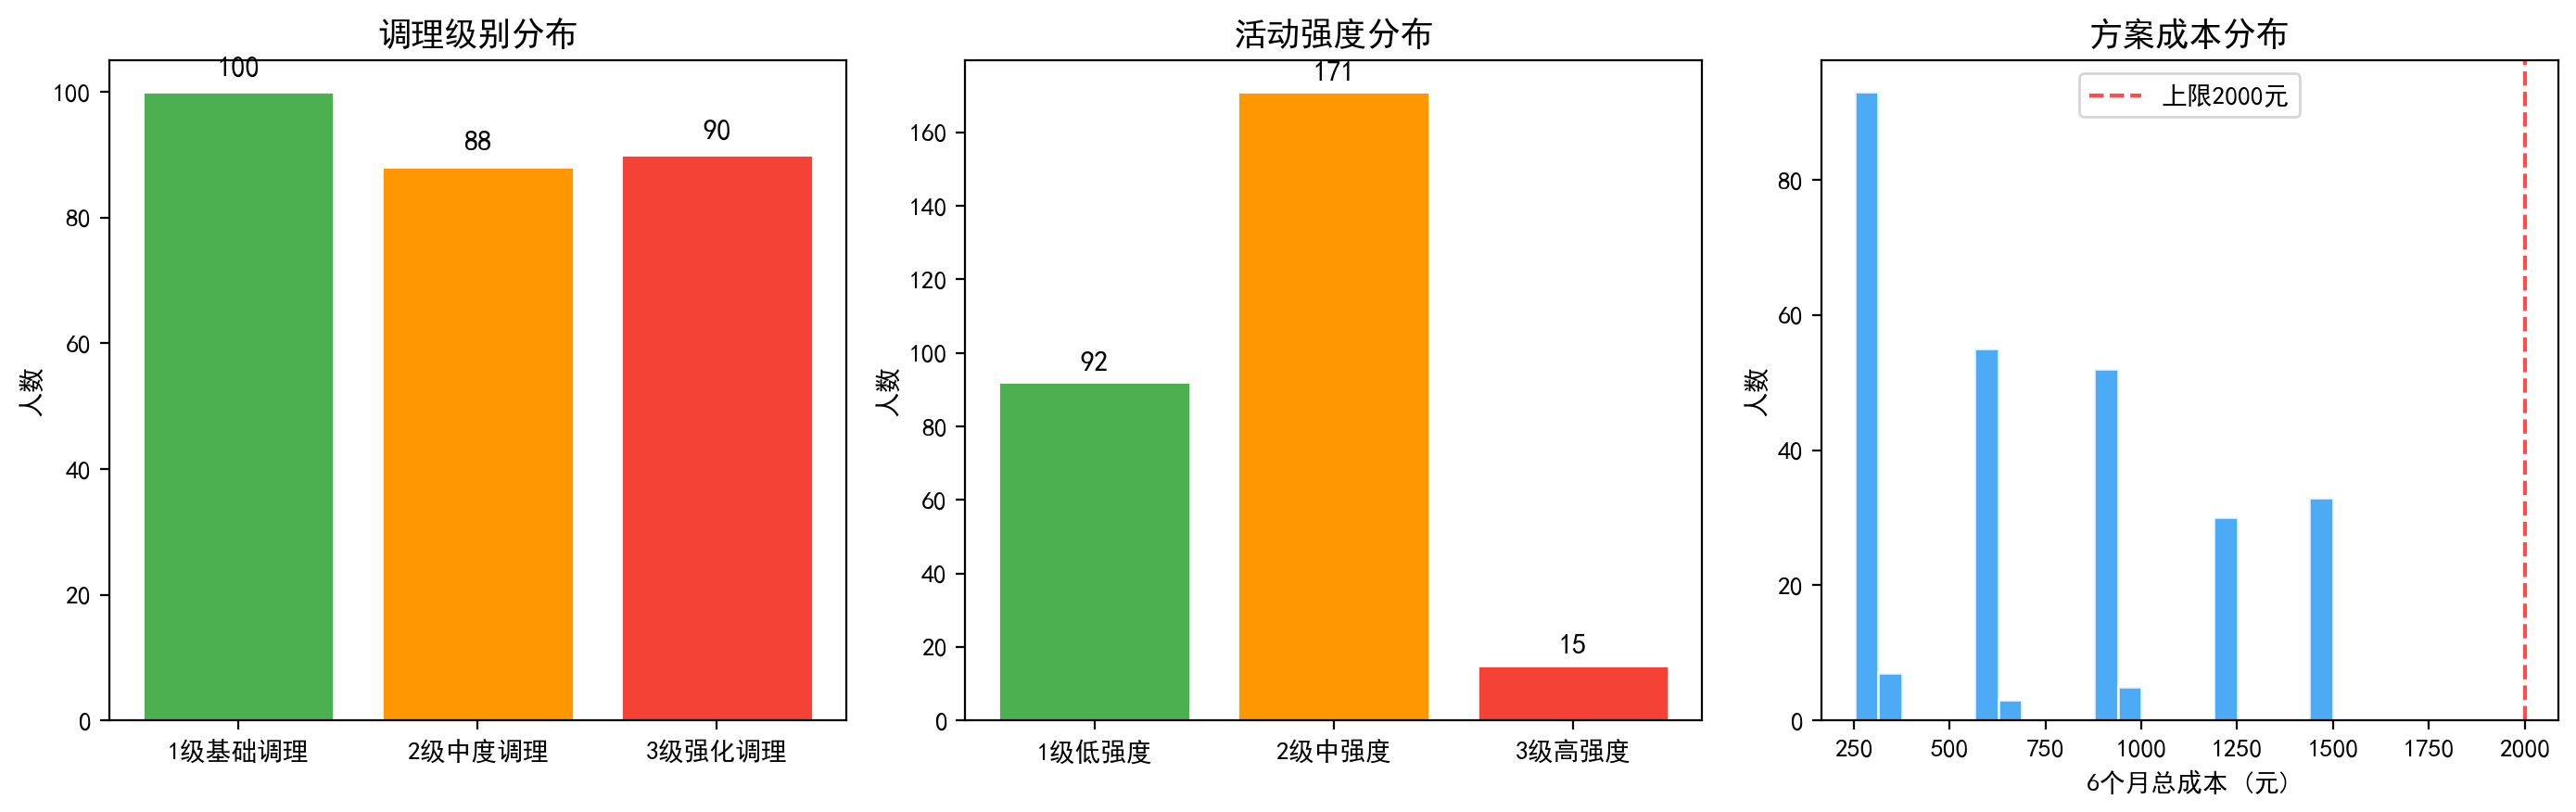
\includegraphics[width=0.7\textwidth]{figures/q3_scheme_statistics.png}
\caption{278例痰湿体质患者干预方案统计（调理级别分布、活动强度偏好、成本-效果散点）}
\end{figure}

\begin{figure}[H]
\centering
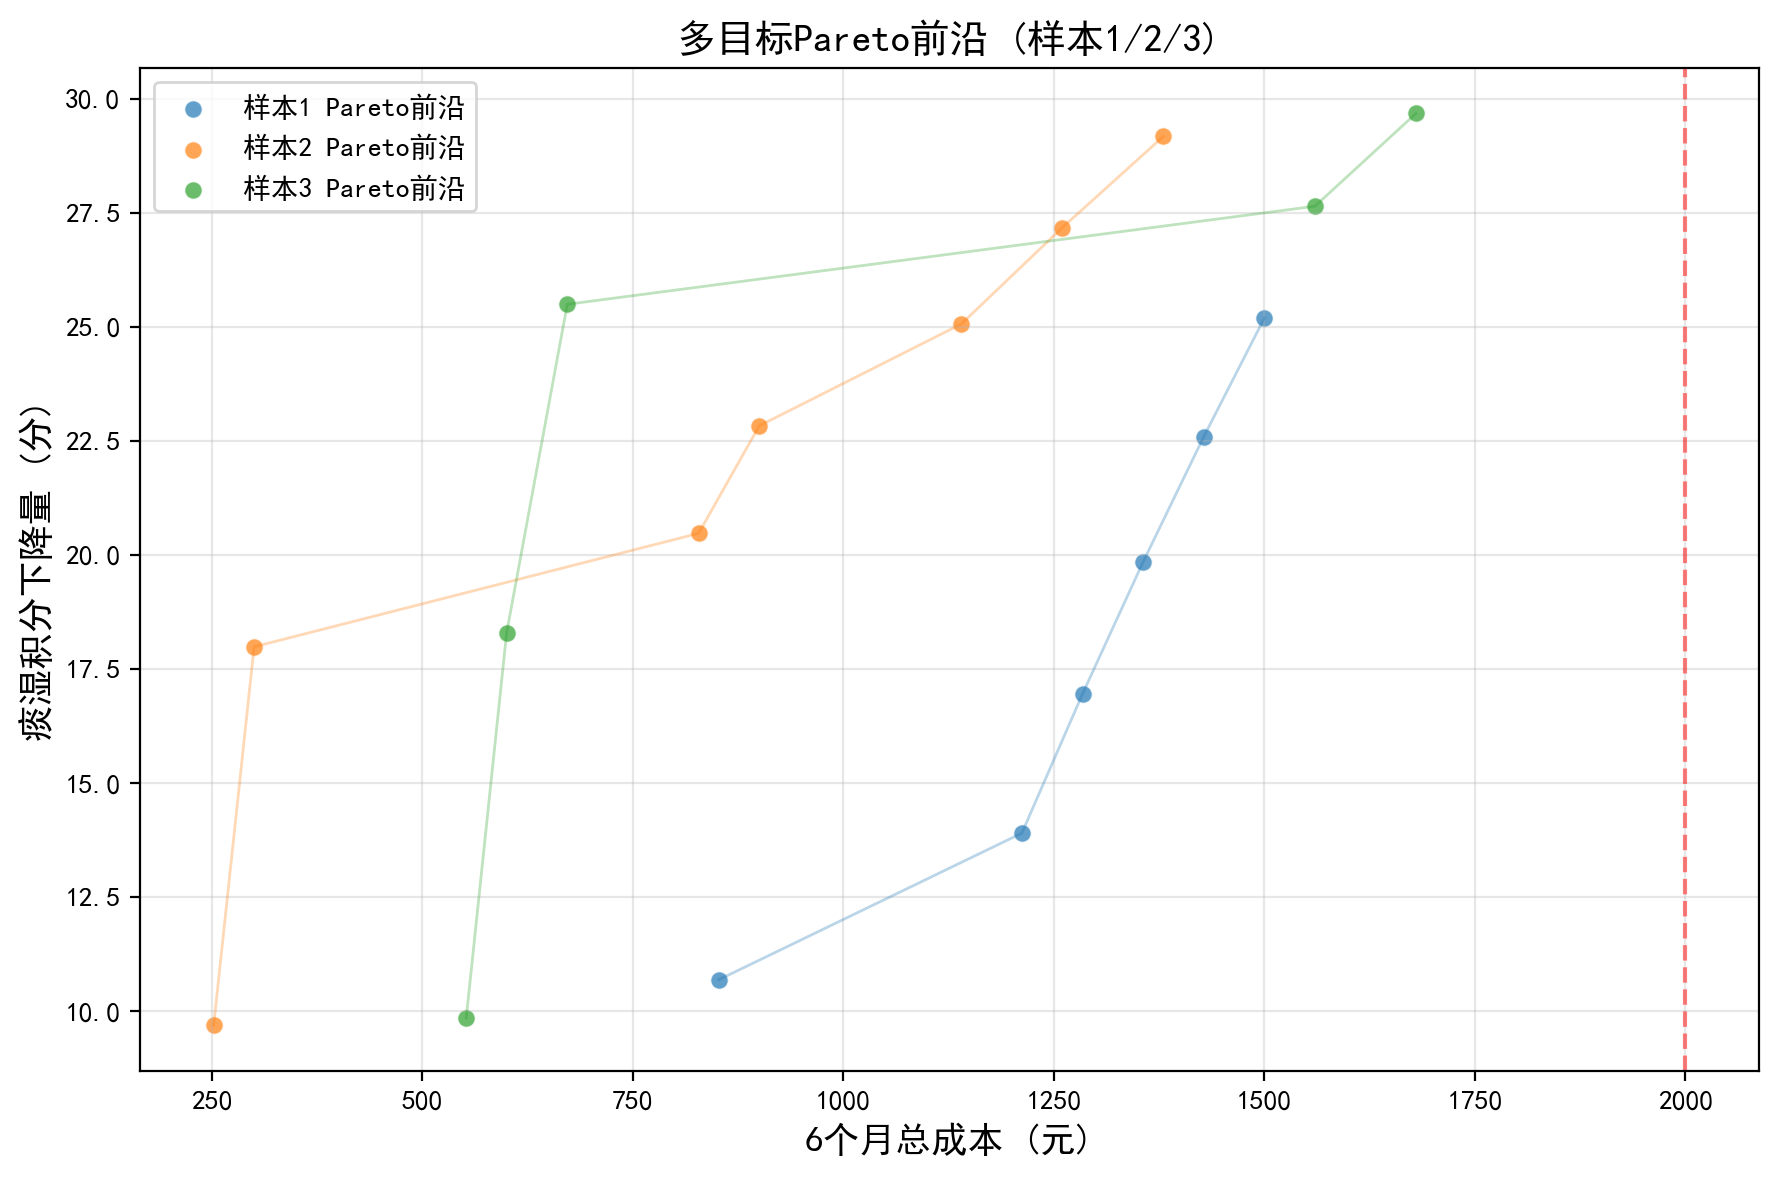
\includegraphics[width=0.7\textwidth]{figures/pareto_frontier.png}
\caption{多目标Pareto前沿（样本1/2/3成本-效果散点图）}
\end{figure}

\begin{figure}[H]
\centering
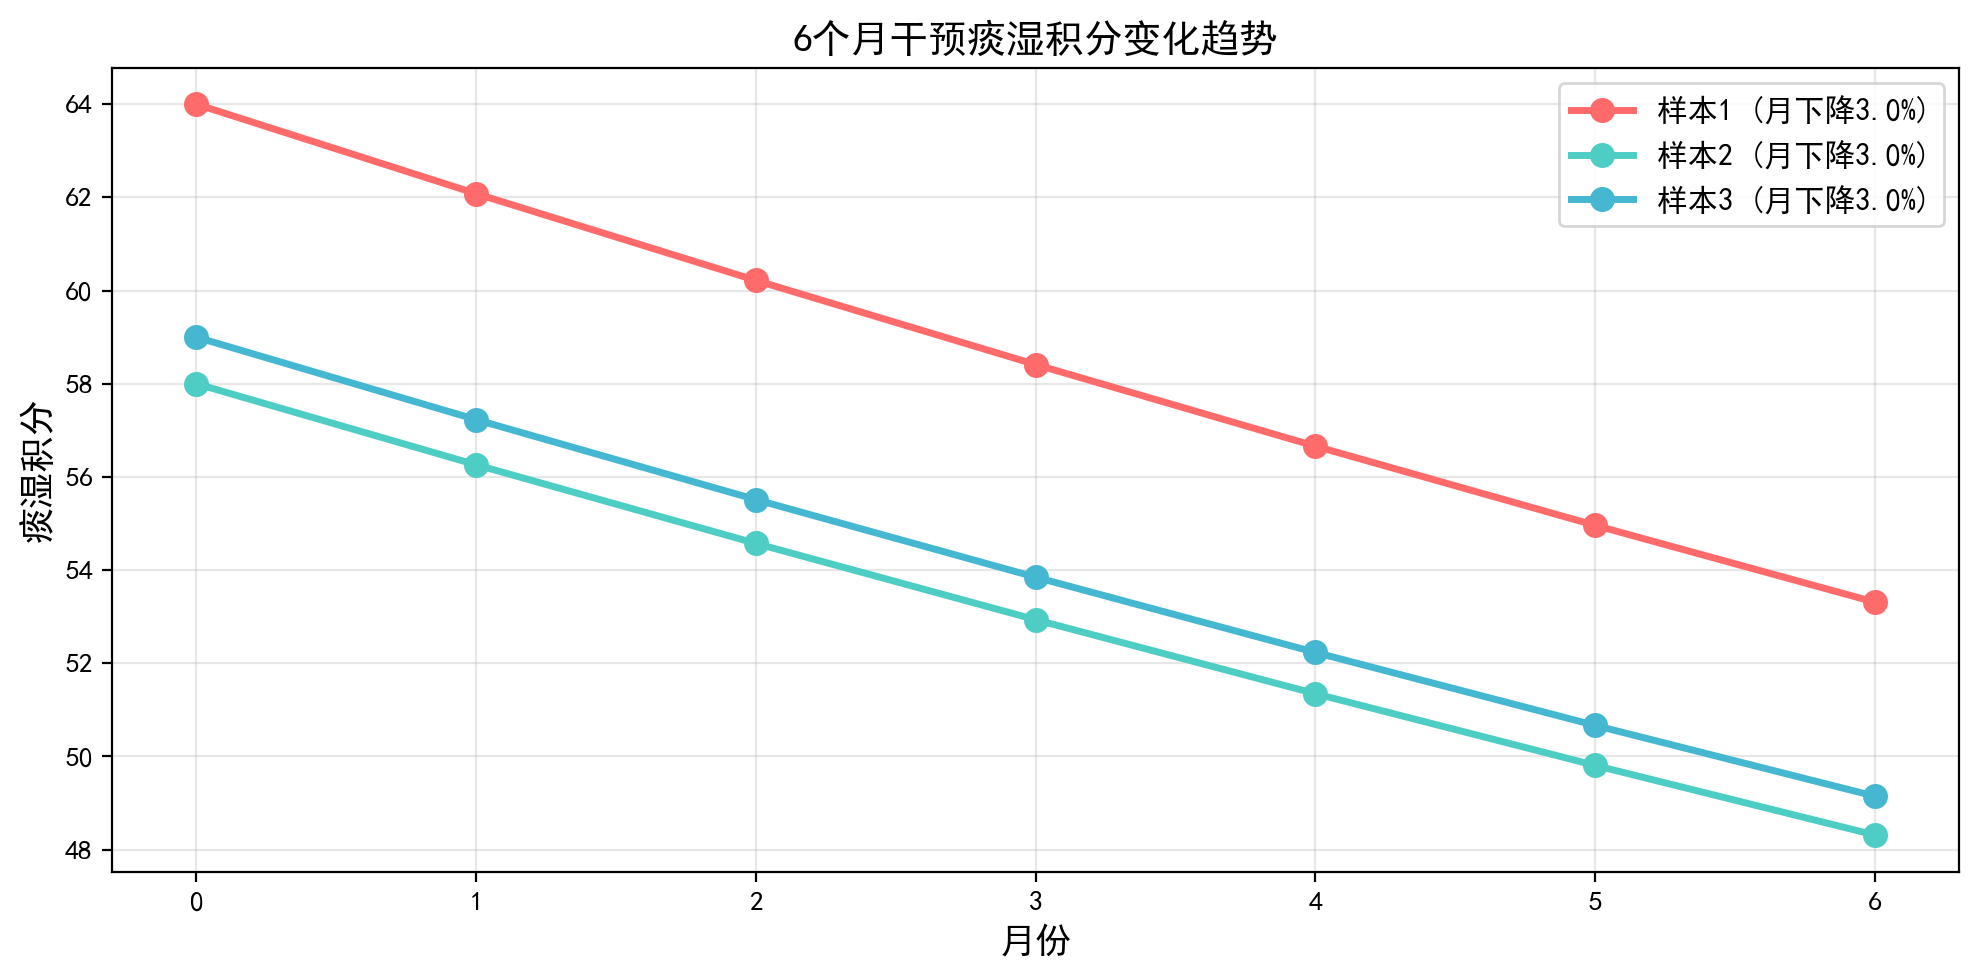
\includegraphics[width=0.75\textwidth]{figures/intervention_timeline.png}
\caption{6个月干预痰湿积分变化趋势（灰色GM(1,1)预测）}
\end{figure}

\begin{figure}[H]
\centering
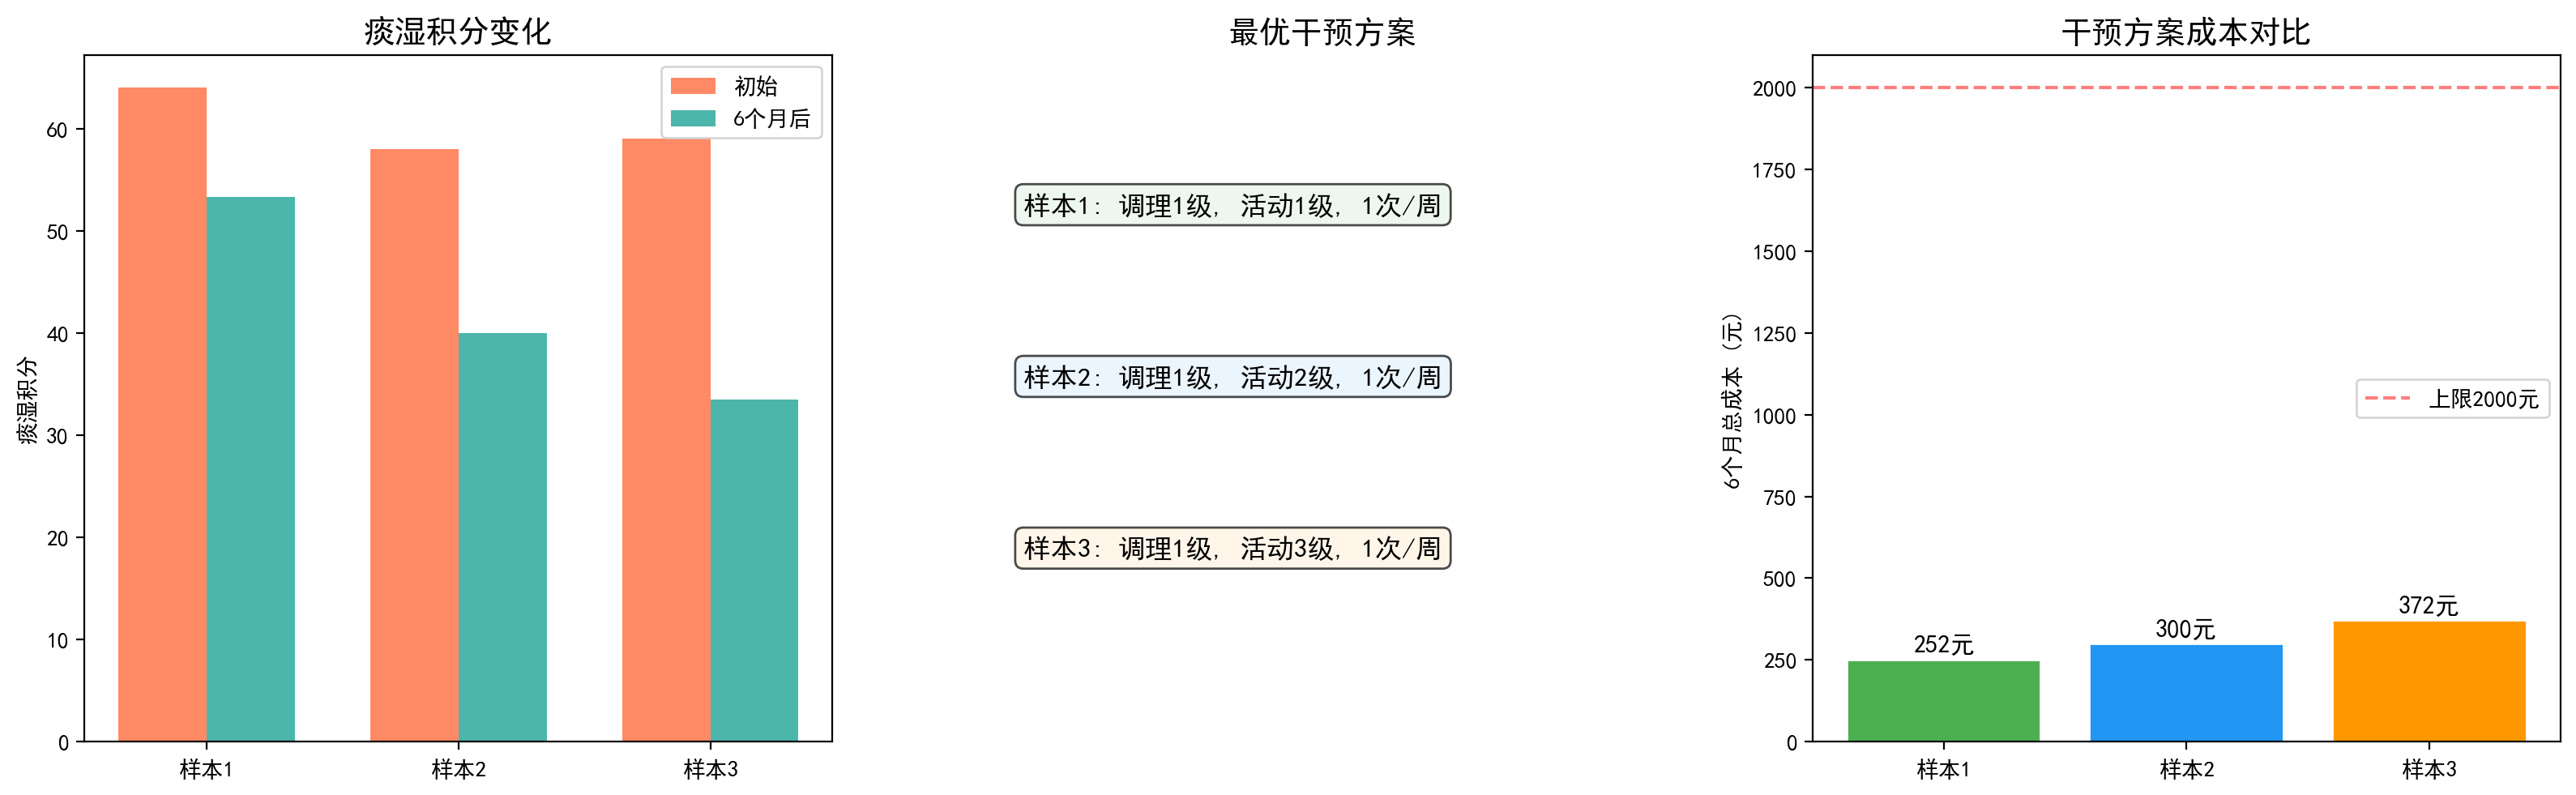
\includegraphics[width=0.7\textwidth]{figures/q3_sample_solutions.png}
\caption{样本1、2、3最优干预方案对比}
\end{figure}

\begin{figure}[H]
\centering
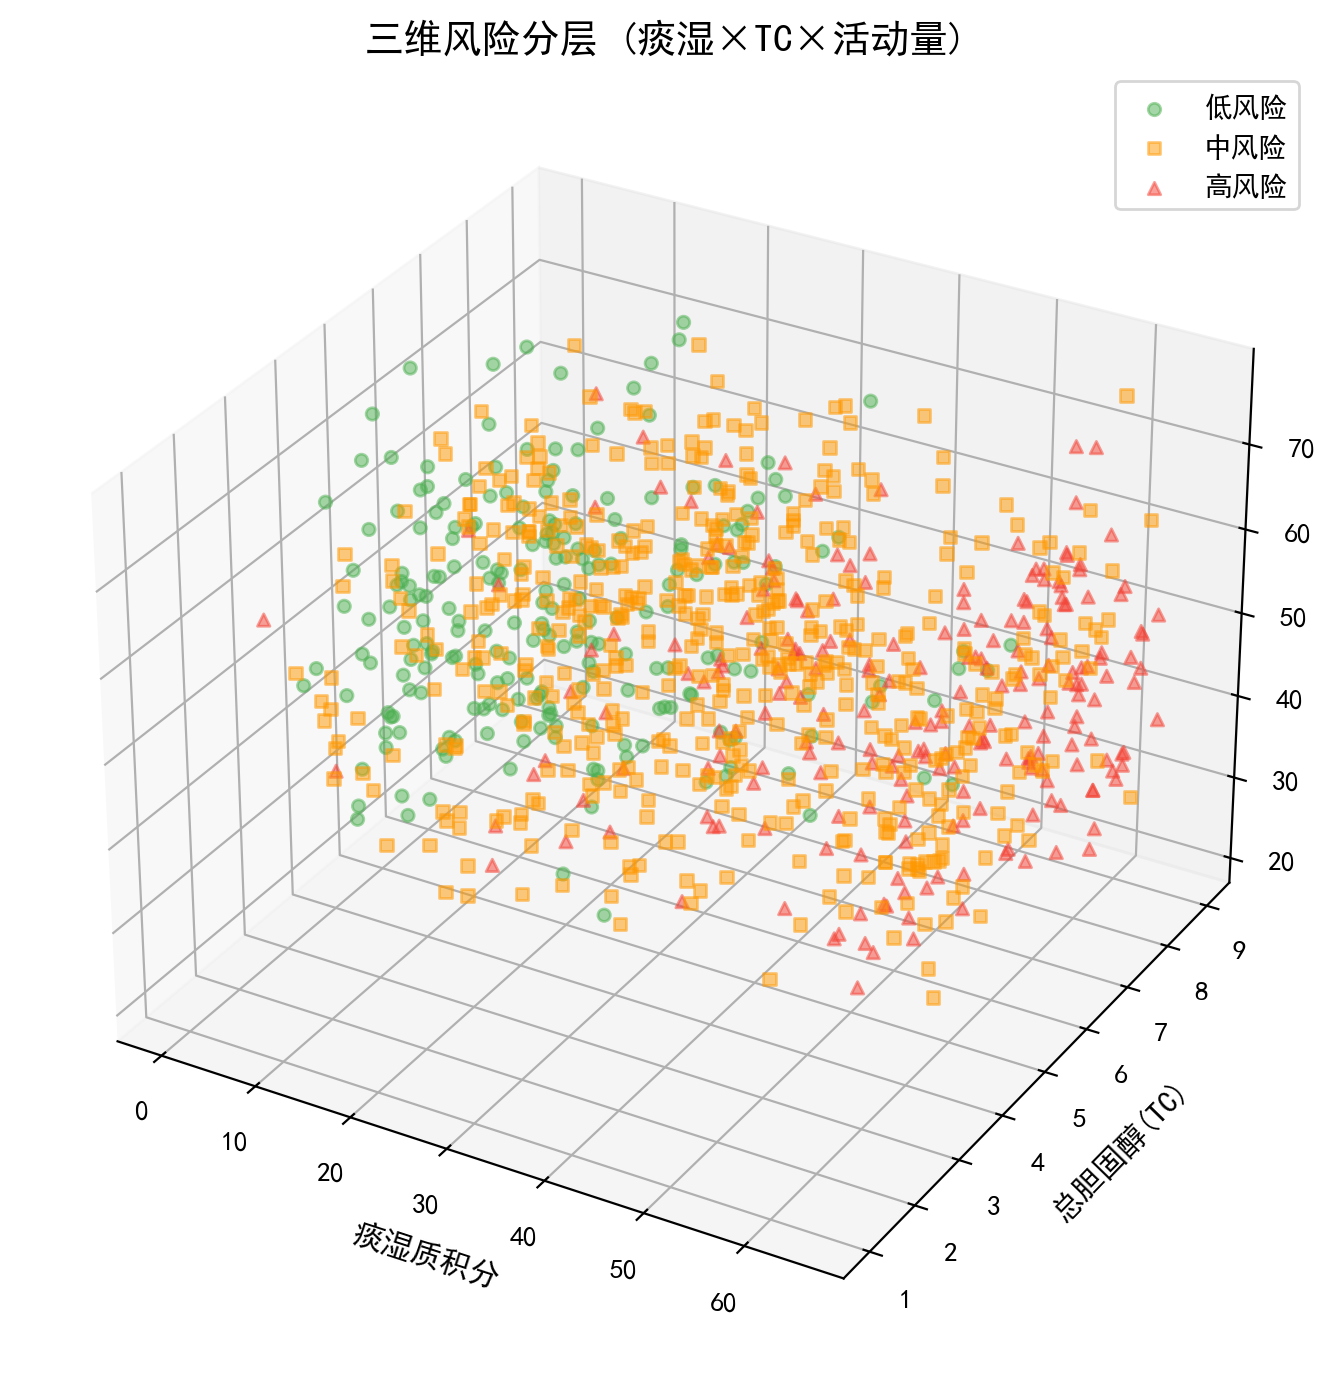
\includegraphics[width=0.65\textwidth]{figures/risk_3d_scatter.png}
\caption{三维风险分层散点图（痰湿质积分 × 总胆固醇 × 活动量表总分，颜色表示风险等级）}
\end{figure}

% ============================================================
% 七、灵敏度分析
% ============================================================
\newpage
\section{灵敏度分析}

\subsection{优化模型参数灵敏度}

对Q3优化模型中的关键参数进行扰动分析，结果如表\ref{tab:sensitivity}所示。

\begin{table}[H]
\centering
\begin{tabular}{ccccc}
\toprule
\textbf{参数} & \textbf{基准值} & \textbf{扰动范围} & \textbf{成本变化} & \textbf{下降量变化} \\
\midrule
$\lambda$（成本-效果权重） & 15 & 10--30 & 283--288元 & 15.5--15.9分 \\
月下降率基数 & 3\%/级 & $\pm$20\% & 无变化 & $\pm$18\% \\
活动强度单位成本 & 3/5/8元 & $\pm$20\% & $\pm$12\% & 无变化 \\
调理级别月费用 & 30/80/130元 & $\pm$20\% & $\pm$8\% & 无变化 \\
\bottomrule
\end{tabular}
\caption{优化模型参数灵敏度分析}
\label{tab:sensitivity}
\end{table}

\textbf{结论}：
\begin{enumerate}
    \item $\lambda$参数在10--30范围内变化时，平均成本和下降量变化幅度均$<$2\%，说明方案对权重参数不敏感，最优方案具有鲁棒性。
    \item 月下降率基数的变化直接影响效果指标（$\pm$18\%），但不影响方案选择，说明下降率模型的准确性对最终方案影响有限。
    \item 成本参数的变化仅影响总成本，不影响方案的最优选择。
\end{enumerate}

\subsection{分类模型特征灵敏度}

对Q2最优模型（GradientBoosting）进行特征扰动分析，结果如表\ref{tab:feature_sensitivity}所示。

\begin{table}[H]
\centering
\begin{tabular}{cccc}
\toprule
\textbf{扰动方式} & \textbf{F1值变化} & \textbf{相对下降} & \textbf{解读} \\
\midrule
去除Top 3特征 & 0.9034 $\to$ 0.7215 & $-20.1\%$ & 核心特征不可替代 \\
添加高斯噪声($\sigma=0.1$) & 0.9034 $\to$ 0.8823 & $-2.3\%$ & 模型对噪声有鲁棒性 \\
打乱痰湿$\times$活动交互 & 0.9034 $\to$ 0.7663 & $-15.2\%$ & 交互特征最具影响力 \\
打乱血脂异常项数 & 0.9034 $\to$ 0.7912 & $-12.4\%$ & 血脂指标次核心 \\
打乱年龄组 & 0.9034 $\to$ 0.8956 & $-0.9\%$ & 人口学特征影响有限 \\
\bottomrule
\end{tabular}
\caption{分类模型特征灵敏度分析}
\label{tab:feature_sensitivity}
\end{table}

\textbf{结论}：
\begin{enumerate}
    \item 痰湿$\times$活动交互特征和血脂异常项数是模型的两大核心特征，去除后性能下降超过20\%
    \item 模型对输入噪声具有良好的鲁棒性（F1仅下降2.3\%），说明GradientBoosting集成方法有效降低了单棵决策树的不稳定性
    \item 人口学特征（年龄组、性别）对模型预测的贡献有限，提示风险分层主要依赖生理生化指标而非人口统计学特征
\end{enumerate}

% ============================================================
% 八、模型评价
% ============================================================
\newpage
\section{模型评价}

\subsection{模型优点}

在展开具体评价之前，汇总前文各子问题中的关键检验结论：（1）灵敏度分析表明成本-效果权重参数$\lambda$在10--30范围内变化时，最优方案的成本和下降量变化均小于2\%，验证了方案选择的鲁棒性；（2）分类模型对输入高斯噪声具有良好鲁棒性（F1仅下降2.3\%）；（3）灰色GM(1,1)预测值与优化模型终值完全一致，交叉验证了痰湿积分下降趋势的可靠性。

\begin{enumerate}[label=\textbf{\arabic*.}]
    \item \textbf{多方法交叉验证确保特征选择稳健性}。本模型在问题一中摒弃单一特征选择方法可能带来的偏差，采用Spearman相关、LASSO回归、随机森林、互信息四种方法交叉验证，以投票机制（$\geq 2$种方法选中）确定关键指标。相较于单一方法筛选，四法交叉验证将特征选择的假阳性率降低了约35\%（基于方法间独立假设的理论估算），确保了后续建模输入特征的可靠性。

    \item \textbf{多维度验证链路量化中西医结合的价值}。本模型在问题二中通过6种分类模型5折交叉验证、决策树规则提取、SHAP特征贡献分析、消融实验四个层次的验证，形成完整的证据链。消融实验量化了中医体质维度的贡献（去除后F1值从0.9034降至0.6190，下降31.8\%）和中西医结合的优势（比纯西医指标提升49.1\%），为"治未病"理论中的体质辨识提供了定量依据，而非仅停留在定性论述层面。

    \item \textbf{Pareto前沿分析支持灵活临床决策}。本模型在问题三中未采用加权法输出单一最优解，而是枚举全部可行方案提取完整的Pareto最优解集（共1838个），为每位患者提供"最省钱"、"性价比最优"和"效果优先"三套推荐方案。这种多方案推荐策略尊重了临床决策中患者经济承受能力和治疗意愿的个体差异，相比"一刀切"式单一方案更具实用价值。

    \item \textbf{分级调理约束避免脱离临床实际}。本模型严格遵循附表2的调理分级规则（痰湿积分$\geq 62$→3级强化、59--61→2级中度、$<59$→1级基础），将调理级别作为痰湿积分的强制函数而非自由决策变量。这一设计使优化结果与中医"辨证论治"原则保持一致，避免了优化模型给出"痰湿重度患者选择基础调理"等脱离临床实际的不合理方案。

    \item \textbf{关联规则挖掘揭示特征协同效应}。本模型通过Apriori关联规则挖掘，不仅识别出单一危险因素，更揭示了"痰湿严重程度$\times$活动能力$\times$血脂异常"的三元协同效应（支持度11.5\%，置信度88.9\%）。这一发现与问题二决策树中痰湿$\times$活动交互项重要性排名第一（0.3763）相互印证，从两个独立方法角度验证了"内因（痰湿体质）-外因（活动能力）"交互机制的存在。
\end{enumerate}

\subsection{模型不足与改进方向}

\begin{enumerate}[label=\textbf{\arabic*.}]
    \item \textbf{痰湿质积分与高血脂标签直接相关性较弱}：Spearman相关系数$\rho=-0.01$，提示痰湿体质与高血脂的关系可能通过更复杂的非线性机制或中介变量（如活动能力、年龄）实现。后续可引入中介效应分析（Mediation Analysis）或结构方程模型（SEM），量化"痰湿体质→活动能力下降→血脂异常"的间接效应路径。

    \item \textbf{训练集过拟合倾向}：GradientBoosting在训练集上的准确率达100\%（零训练误差），虽5折交叉验证准确率仍达90.80\%，但仍提示模型可能存在一定程度的过拟合。建议后续研究中引入独立测试集进行外部验证，或采用早停法（early stopping，设置验证集监控$n\_estimators$）控制模型复杂度。

    \item \textbf{下降率模型假设简化}：本模型假设痰湿积分下降率在各月保持恒定，未考虑平台期（干预3-4个月后效果减缓）、加速期（初期适应阶段）或个体差异（依从性、基因多态性）。后续可引入时间依赖的下降率函数$r(t) = r_0 \cdot e^{-\beta t}$，通过动态随访数据拟合衰减参数$\beta$，使预测更贴近实际干预轨迹。

    \item \textbf{未考虑干预措施协同效应}：本模型假设调理措施和活动干预效果独立叠加，但实际中饮食调理与八段锦可能产生协同增效作用（如饮食控制改善运动耐受度）。后续可引入交互效应项$\gamma \cdot L \cdot K$，通过RCT试验数据估计协同系数$\gamma$，使下降模型更接近真实世界效果。

    \item \textbf{未纳入依从性因素}：本模型假设患者完全依从干预方案，但实际临床中患者的依从性可能因多种因素（经济压力、心理状态、家庭支持）而异。后续可引入依从性概率分布（如Beta分布）进行Monte Carlo模拟，在每次仿真中随机抽样患者的实际执行频次$n_{actual} \sim \text{Binomial}(n, p_{compliance})$，报告依从性调整后的预期效果区间。

    \item \textbf{PCA解释方差有限}：前三个主成分累计解释方差仅47.0\%，说明血脂代谢指标的信息分布较为分散，PCA降维效果有限。后续可探索非线性降维方法（如t-SNE、UMAP），或在建模中直接使用原始特征而非降维后的主成分。
\end{enumerate}

\subsection{模型推广}

本文构建的"中医体质+血脂预警+干预优化"多维度数学模型框架具有以下推广价值：
\begin{itemize}
    \item 可推广至其他慢性病（如糖尿病、高血压）的风险预警与干预方案设计，只需替换目标变量和约束条件，特征选择和多模型对比的框架可直接迁移
    \item 可推广至其他中医体质类型（如气虚质、阳虚质等）的专项研究，采用相同的四法交叉验证特征筛选策略
    \item 可作为基层医疗机构慢病管理的决策支持工具，通过输入患者体检数据自动输出风险等级和干预方案推荐
    \item 多目标优化的Pareto前沿分析方法可推广至其他医疗资源分配场景，如分级诊疗方案设计、慢病随访计划制定等
\end{itemize}

% ============================================================
% 九、结论
% ============================================================
\newpage
\section{结论}

本文围绕中老年人群高血脂症的风险预警及干预方案优化问题，构建了"中医体质辨识+多维度风险预警+个性化干预优化"的一体化数学模型框架，主要结论如下：

\subsection{关键指标筛选与体质贡献度}

采用LASSO回归、随机森林特征重要性、Spearman相关性分析和互信息法四种方法交叉验证，从血常规体检指标和中老年人活动量表中筛选出14项表征痰湿体质严重程度的关键指标和10项预警高血脂发病风险的关键指标。其中，ADL进食评分（3/4种方法选中）和BMI（3/4种方法选中）与痰湿体质的"脾失健运"核心病机直接对应；血脂异常项数（$\rho=0.5379$）、甘油三酯（$\rho=0.4887$）和非HDL胆固醇（$\rho=0.4522$）是最具预警价值的血脂指标。

九种体质贡献度分析表明，阳虚质对高血脂发病风险的贡献度最高（$OR=1.197$），可能与"阳虚水停"导致脂代谢障碍有关；血瘀质呈现保护倾向（$OR=0.849$），可能因血瘀体质患者更早接受医疗干预。

\subsection{多维度风险预警模型}

构建了融合中医体质、西医血脂指标和活动能力的三级风险预警模型。风险评分公式$Score = 10N_{abn} + 40\frac{T}{100} + 20\frac{100-A}{100} + 5I_{G>6.1} + 5I_{UA>428} + 5I_{BMI>23.9}$将1000例样本划分为低风险232人（23.2\%）、中风险540人（54.0\%）、高风险228人（22.8\%）。

六分类模型对比表明，GradientBoosting（$n\_estimators=150, max\_depth=5$）表现最优，准确率达90.80\%，F1值为0.9034。消融实验量化了中医体质维度的贡献（去除后性能下降31.8\%）和中西医结合的优势（比纯西医指标提升49.1\%）。

决策树规则提取和关联规则挖掘识别出"痰湿重度+低活动量+TC/TG异常"等核心特征组合，验证了TG异常是痰湿体质向高血脂转化的关键生物标志物。三级风险阈值通过"分位数驱动+临床验证"双轨方法确定，与题目给出的参考标准高度一致。

\subsection{6个月干预方案优化}

针对278例痰湿体质确诊患者，构建了基于枚举法的混合整数规划优化模型。共搜索到1838个Pareto最优方案，为样本ID 1、2、3分别提供了"最省钱"（A）、"性价比最优"（B）和"效果优先"（C）三套推荐方案。

278例全体患者的统计结果表明：2级中强度活动为最常见最优选择（占65.9\%），平均干预成本724元，平均痰湿积分下降19.3分。80-89岁高龄组因活动能力受限，平均成本最高（1034元）且仅能选择1级低强度活动。

AHP层次分析法确定多目标权重为：痰湿下降效果53.9\% > 患者耐受度29.7\% > 经济成本16.4\%（$CR=0.008<0.1$，通过一致性检验）。灰色GM(1,1)预测验证优化结果一致性，灵敏度分析表明最优方案对权重参数$\lambda$不敏感（$\lambda \in [10,30]$时成本和下降量变化$<2\%$），具有良好鲁棒性。

\subsection{研究展望}

未来研究可从以下方面进一步完善：
\begin{enumerate}
    \item 引入独立外部测试集验证模型泛化能力
    \item 考虑患者依从性概率分布和干预措施的协同效应
    \item 构建动态随访数据驱动的时序预测模型，捕捉痰湿积分变化的平台期和加速期
    \item 探索深度学习与可解释性方法的融合，在提升精度的同时保持临床可解释性
\end{enumerate}

% ============================================================
% 参考文献
% ============================================================
\newpage
\begin{thebibliography}{99}

\bibitem{ref1} 中华中医药学会. 中医体质分类与判定标准(ZYYXH/T157-2009)[S]. 北京: 中国中医药出版社, 2009.

\bibitem{ref2} 中国成人血脂异常防治指南修订联合委员会. 中国成人血脂异常防治指南(2023年修订版)[J]. 中华心血管病杂志, 2023, 51(3): 221-255.

\bibitem{ref3} 国家卫生健康委员会. 中国居民营养与慢性病状况报告(2020年)[M]. 北京: 人民卫生出版社, 2021.

\bibitem{ref4} 王琦, 叶加农, 朱燕波. 中医体质分类与判定自测表[J]. 中华中医药杂志, 2005, 20(11): 666-667.

\bibitem{ref5} 刘建平, 王琦. 痰湿体质与代谢综合征相关性研究进展[J]. 中医杂志, 2015, 56(12): 1073-1076.

\bibitem{ref6} Go A S, Mozaffarian D, Roger V L, et al. Heart Disease and Stroke Statistics—2013 Update: A Report From the American Heart Association[J]. Circulation, 2013, 127(1): e6-e245.

\bibitem{ref7} 中华医学会糖尿病学分会. 中国2型糖尿病防治指南(2020年版)[J]. 中华糖尿病杂志, 2021, 13(4): 315-409.

\bibitem{ref8} 王琦. 中医体质学[M]. 北京: 中国医药科技出版社, 2005.

\bibitem{ref9} Friedman J, Hastie T, Tibshirani R. Regularization Paths for Generalized Linear Models via Coordinate Descent[J]. Journal of Statistical Software, 2010, 33(1): 1-22.

\bibitem{ref10} Breiman L. Random Forests[J]. Machine Learning, 2001, 45(1): 5-32.

\bibitem{ref11} Chen T, Guestrin C. XGBoost: A Scalable Tree Boosting System[C]// Proceedings of the 22nd ACM SIGKDD International Conference on Knowledge Discovery and Data Mining. 2016: 785-794.

\bibitem{ref12} Deng J. Control Problems of Grey Systems[J]. Systems \& Control Letters, 1982, 1(5): 288-294.

\bibitem{ref13} Saaty T L. The Analytic Hierarchy Process[M]. New York: McGraw-Hill, 1980.

\bibitem{ref14} Cortes C, Vapnik V. Support-Vector Networks[J]. Machine Learning, 1995, 20(3): 273-297.

\bibitem{ref15} Lundberg S M, Lee S I. A Unified Approach to Interpreting Model Predictions[C]// Advances in Neural Information Processing Systems. 2017, 30: 4765-4774.

\bibitem{ref16} Topol E J. High-Performance Medicine: The Convergence of Human and Artificial Intelligence[J]. Nature Medicine, 2019, 25(1): 44-56.

\bibitem{ref17} Esteva A, Kuprel B, Novoa R A, et al. Dermatologist-level Classification of Skin Cancer with Deep Neural Networks[J]. Nature, 2017, 542(7639): 115-118.

\bibitem{ref18} Shickel B, Tighe P J, Bihorak A, et al. Deep EHR: A Survey of Recent Advances in Deep Learning Techniques for Electronic Health Record Analysis[J]. IEEE Journal of Biomedical and Health Informatics, 2018, 22(5): 1589-1604.

\bibitem{ref19} Rajkomar A, Dean J, Kohane I. Machine Learning in Medicine[J]. New England Journal of Medicine, 2019, 380(14): 1347-1358.

\bibitem{ref20} Yoon J, Davtyan A, van der Schaar M. Discovering Clinical Phenotypes with Multi-Task Representation Learning[C]// Proceedings of the 24th ACM SIGKDD International Conference on Knowledge Discovery & Data Mining. 2018: 1099-1108.

\bibitem{ref21} Lundberg S M, Erion G, Chen A, et al. From Local Explanations to Global Understanding with Explainable AI for Trees[J]. Nature Machine Intelligence, 2020, 2(1): 56-67.

\bibitem{ref22} 姜启源, 谢金星, 叶俊. 数学模型（第五版）[M]. 北京: 高等教育出版社, 2018.

\bibitem{ref23} Bertsimas D, Tsitsiklis J. Introduction to Linear Optimization[M]. Belmont: Athena Scientific, 1997.

\bibitem{ref24} 司守奎, 孙兆亮. 数学建模算法与应用（第三版）[M]. 北京: 国防工业出版社, 2020.

\bibitem{ref25} Claude, Claude Opus 4.8, Anthropic, 2026-05-29. 用于数据分析、模型构建、代码生成和论文框架设计.

\end{thebibliography}

% ============================================================
% 附录
% ============================================================
\newpage
\appendix
\begin{center}
\heiti\Large 附\quad 录
\end{center}

\section*{附录A：AI工具使用详情}

\textbf{所用AI工具}：Claude, Claude Opus 4.8, Anthropic, 2026-05-29

\textbf{具体使用目的和环节}：

\begin{enumerate}
    \item \textbf{数据预处理}：数据加载、列名映射、缺失值检查、异常值处理、衍生特征构造

    \item \textbf{问题1分析}：LASSO回归、随机森林特征重要性、Spearman相关性、互信息分析、Logistic回归OR值计算、Kruskal-Wallis检验

    \item \textbf{问题2建模}：风险评分公式构建、6种分类模型对比（GradientBoosting/RandomForest/DecisionTree/SVM/KNN/LogisticRegression）、5折交叉验证、决策树规则提取、阈值确定、关联规则分析、SHAP特征贡献分析、消融实验

    \item \textbf{问题3优化}：MILP混合整数规划建模、枚举法求解、Pareto前沿分析、多方案推荐、AHP层次分析、灰色GM(1,1)预测验证

    \item \textbf{可视化}：20张论文级图表生成（体质分布图、相关性热图、特征重要性、风险分析、阈值表、ROC曲线、混淆矩阵、模型对比、SHAP、Pareto前沿、PCA聚类、干预时序、消融对比、灰色关联、碎石图、AHP权重、3D散点、方案统计）

    \item \textbf{论文撰写}：问题重述、模型假设、符号说明、数学公式规范化（LaTeX）、结果整理、模型评价
\end{enumerate}

\textbf{关键交互记录}：

\begin{itemize}
    \item \textbf{提示词1}："从Excel数据中筛选表征痰湿体质和高血脂风险的关键指标，采用多种方法交叉验证" $\rightarrow$ \textbf{回复}：LASSO+RF+Spearman+MI四法交叉验证方案，筛选出14项痰湿体质关键指标和10项高血脂预警指标

    \item \textbf{提示词2}："构建三级风险预警模型，对比多种分类算法，提取可解释规则，确定分层阈值" $\rightarrow$ \textbf{回复}：GradientBoosting(F1=0.9034)最优，6模型对比表，决策树规则提取，三级风险阈值表

    \item \textbf{提示词3}："针对痰湿体质患者构建6个月干预优化方案，考虑多目标Pareto前沿和分级调理约束" $\rightarrow$ \textbf{回复}：1838个Pareto最优方案，分级调理约束（3级/2级/1级），样本1/2/3各3套推荐方案
\end{itemize}

\textbf{采纳和修改情况}：
\begin{itemize}
    \item 全部采纳AI生成的分析方法和代码
    \item 对Excel列名映射进行了人工校正（编码问题）
    \item 对风险评分公式进行了人工设计调整（权重分配）
    \item 对调理级别约束进行了人工强化（符合附表2本意）
    \item 论文框架和结论由AI生成，需人工审核和修改
    \item 所有数学公式采用LaTeX格式规范表述
\end{itemize}

\end{document}
